% !TeX spellcheck = de_DE
\chapter{\IfLanguageName{dutch}{Stand van zaken}{State of the art}}
\label{ch:stand-van-zaken}

% Tip: Begin elk hoofdstuk met een paragraaf inleiding die beschrijft hoe
% dit hoofdstuk past binnen het geheel van de bachelorproef. Geef in het
% bijzonder aan wat de link is met het vorige en volgende hoofdstuk.

% Pas na deze inleidende paragraaf komt de eerste sectiehoofding.

Dit hoofdstuk bevat de literatuurstudie omtrend het onderwerp. Hier wordt de architectuur en termen uitgelegd. Ook zal hier een vergelijking gemaakt worden tussen onderdelen van microservices. Een duidelijk beeld van een order-to-cash proces zal hier ook gemaakt worden.

\section{Microservices}
\subsection{Definitie}
Een term die vaak zal terug keren in deze paper is 'monolithic'. "Monolithic software is designed to be self-contained; components of the program are interconnected and interdependent rather than loosely coupled as is the case with modular software programs." \textcite{Wigmore2016}.
Om te begrijpen waarom een overschakeling naar microservices een goed idee is, kaarten we de moeilijkheden bij monolithic architectuur aan. Bij een verandering binnen een monolithic architectuur, wordt er een heel nieuwe versie van de architectuur uitgebracht. Een verandering brengt een hoop extra werk mee \textcite{Mauersberger2017}. Dit omvat 
\begin{itemize}
	\item De volledige architectuur moet opnieuw getest worden.
	\item Deze architectuur kan heel complex worden bij het toevoegen van functionaliteiten.
	\item De complete architectuur moet opnieuw gedeployed worden bij elke update.
	\item De impact van een verandering kan verkeerd ingeschat worden.
	\item Bij een fout in een proces, kan de volledige architectuur falen.
\end{itemize}
De definitie die te vinden is in dit artikel, gaat als volgt: "A method of developing software applications as a suite of independently deployable, small, modular services in which each service runs a unique process and communicates through a well-defined, lightweight mechanism to serve a business goals.". Als je de definitie leest, zie je drie onderdelen. Het eerste onderdeel vertelt hoe een microservice in elkaar zit. Het is een onafhankelijke, kleine, modulaire services. Modulaire services zijn services waarbij veel delen uitwisselbaar zijn met diverse services. De services staan los van elkaar. Ze hebben geen invloed op elkaar. Daarom zijn ze ook onafhankelijk. Wordt er info gestuurd of gevraagd van services A dan zal dit geen invloed hebben op de andere services. De eenvoudige communicatie is een tweede eigenschap van microservices. Er is nood aan communicatie omdat sommige services wel data moeten uitwisselen om hun 'job' te kunnen doen. De communicatie kan gebeuren op verschillende manier. De manier die gekender is, is 'Messaging via a Message Broker'. Dit wil zeggen dat microservice A een bericht plaats op de wachtrij bij microservice B wanneer die data wil doorsturen. Dan kan microservices B aan die data wanneer hij die nodig heeft. Ze zullen soms moeten wachten maar ze zijn zo goed als onafhankelijk van elkaar. De derde eigenschap omvat dat een microservice wordt gemaakt in functie van een requirement uit de business. Elk product in de business heeft een doel dat moet voldoen aan eisen. Het unieke aan microservices is dat we ze gaan bekijken vanuit de eisen binnen de business. Het doel van microservices is, de problemen die te vinden zijn bij een monolithic, verhelpen. De vorige definite legde uit wat microservices zijn. Dit artikel zegt waar men microservices kan plaatsen. Er is dus één groot framework. Daar zitten meerdere onafhankelijke services in.

\begin{figure}[h]
	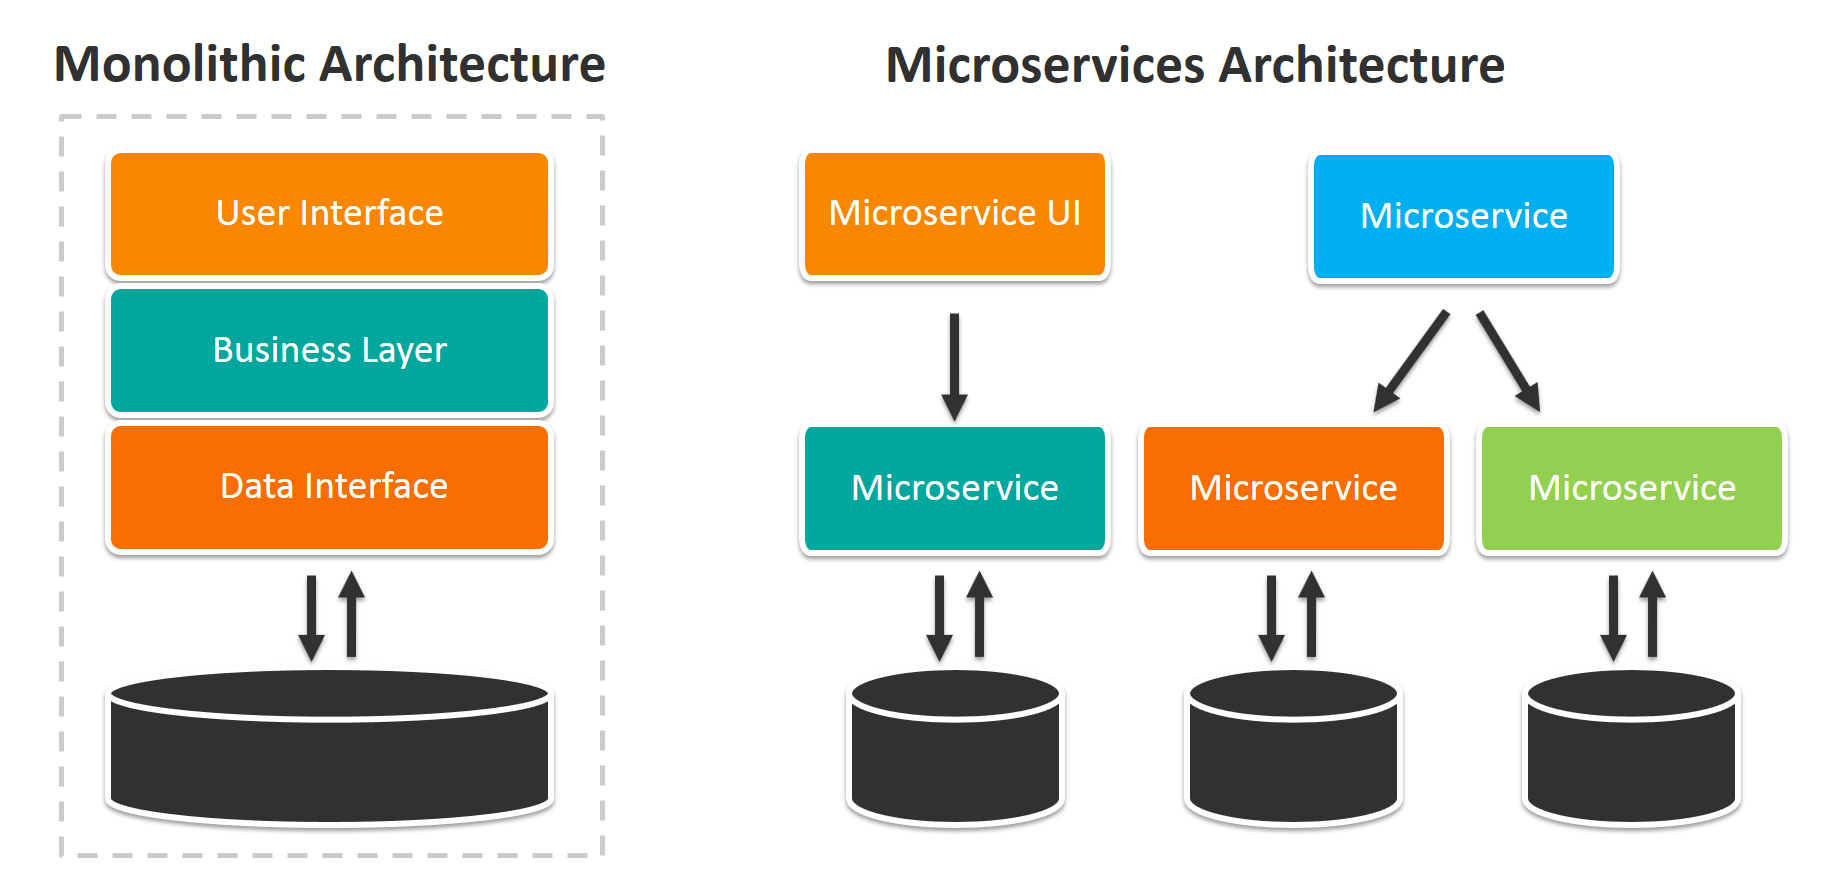
\includegraphics[width=10cm]{microservices-vs-monolithic.jpg}
	\centering
	\caption{Een monolithic architectuur naast een microservice architectuur. \textcite{Watts2018}}
\end{figure}
Zoals te zien in figuur 2.1, \textcite{Watts2018}, is er een groot verschil tussen een monolithic architectuur en die van een microservice. De monolithic wordt weergegeven in de linkerkant van de foto. Aan de rechterkant van de foto is een voorbeeld te zien van een microservice architectuur. Daar is duidelijk te zien dat elke microservice een eigen databank/datastore heeft. Voor elke functionaliteit wordt een microserives aangemaakt, die dan nog eens apart een databank voor zich krijgt. Als bij microservice A een probleem is dan heeft dit niet meteen impact op de andere services. De communicatie tussen microservice A en de anderen zal wel hinder ondervinden. Maar de andere microservices kunnen wel nog steeds onafhankelijk verder. 
Een andere definitie van microservices is: "A software architecting pattern that allows software to be developed into relatively small, distinct components. Each of the components is abstracted by an API(s) and provides a distinct subset of the functionality of the entire application". Ook hier zien we weer het puntje passeren dat een microservice een klein componentje is van een groter geheel. Die eigenschap wordt heel hard benadrukt. Na het uitleggen van microservices, schrijven ze ook over hoe microservices zo scalable zijn. Met scalable bedoelen ze schaalbaarheid. De mogelijkheid van software om mee te groeien als het aantal gebruikers vermeerderd. Dus eigenlijk dat de software nog steeds even goed presteerd bij 10 gebruikers als bij 2 000 gebruikers. Ook lichten ze toe hoe belangrijk API's zijn binnen een microservice architectuur. API's zijn een set van definities die ervoor zorgen dat deeltjes in een programma met elkaar kunnen communcieren. Een voordeel van API's is dat je niet moet weten hoe de andere code werkt. Verder wordt er ook gepraat over de verschillen tussen een monolithic architectuur en een microservice architectuur \textcite{series2018}.


 Zoals te zien is in figuur 2.2. We zien dat de monolithic alle puntjes in een kader heeft. Dit staat symbolisch voor het grote geheel dat eigen is aan een monolithic. Alles zit samen in één grote doos. Maar bij microservices is dit niet zo, daar zit elk deeltje/requirement in een aparte doos \textcite{Benetis2016a} . 
\begin{figure}[h]
	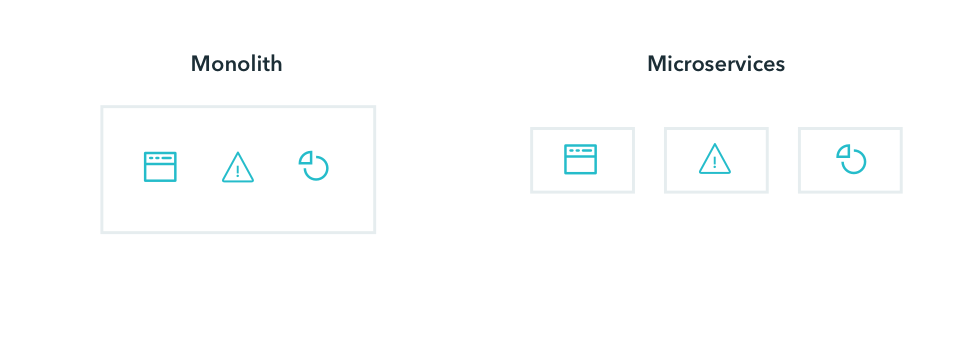
\includegraphics[width=10cm]{Mono_Micro.png}
	\centering
	\caption{Een monolithic vergeleken met een microservice. \textcite{Benetis2016a}}
\end{figure}

In figuur X is duidelijk te zien hoe microservices een website pagina opuvllen.
\begin{figure}[h]
	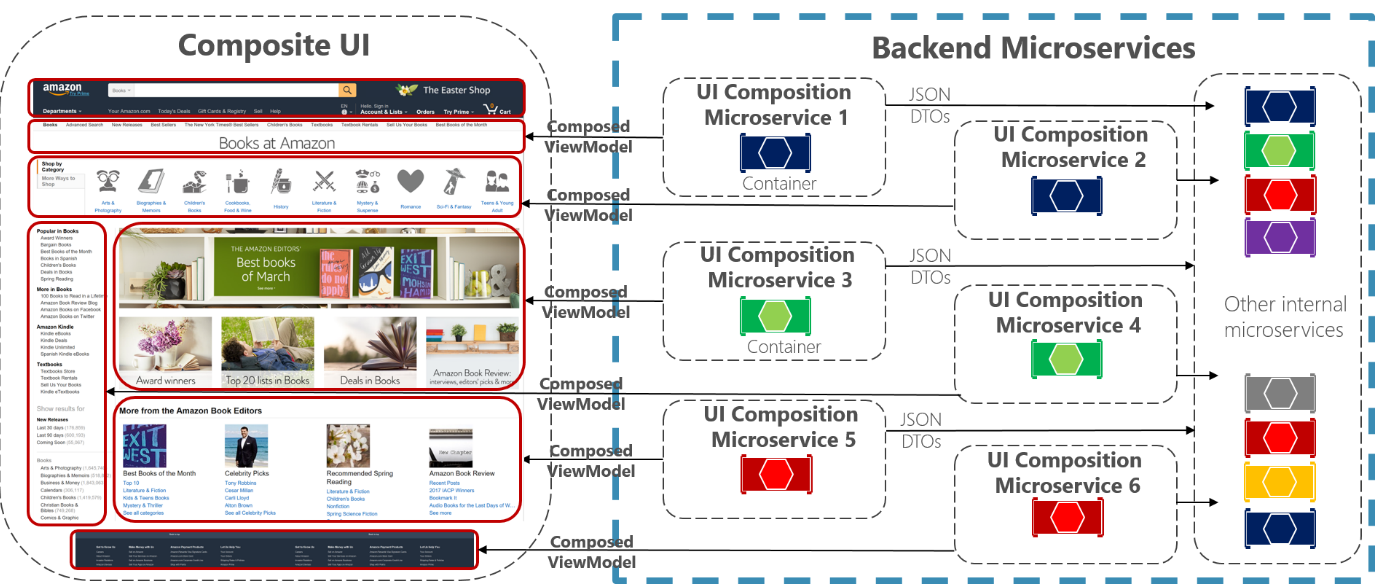
\includegraphics[width=10cm]{microservicesWebsite.png}
	\centering
	\caption{Microservices die de inhoud op een site invullen. \textcite{Koukia2018}}
\end{figure}
De site bestaat uit zes onderdelen. Die onderdelen zijn allemaal dynamisch en ze halen hun info uit databanken. Bij het laden van de pagina gaat elk onderdeeltje zijn info gaan opvragen. Omdat dit allemaal met microservices gebeurt, wordt de info gelijktijdig opgehaald. Ook zullen ze niet moeten wachten op elkaar, tot de een info heeft ontvangen om dan naar de volgende zijn benodigde info te sturen. Elk spreekt zijn eigen databank aan. De microservices die de website opvullen, die kunnen onderliggend ook nog andere microservices aanspreken. Bijvoorbeeld: Een klant is aangemeld op de website van Amazon. De authenticatie microservices zorgt ervoor dat alle microservices weten dat die bepaalde persoon is aangemeld. Dan bij het inladen van voorkeuren of 'soort gelijke producten', kan de microservices die die sectie moet opvullen, vragen aan een andere microservice om de voorkeuren te laten genereren. \textcite{Koukia2018}.

Een voorbeeld van een algemene architectuur is te zien op figuur X.
\begin{figure}[h]
	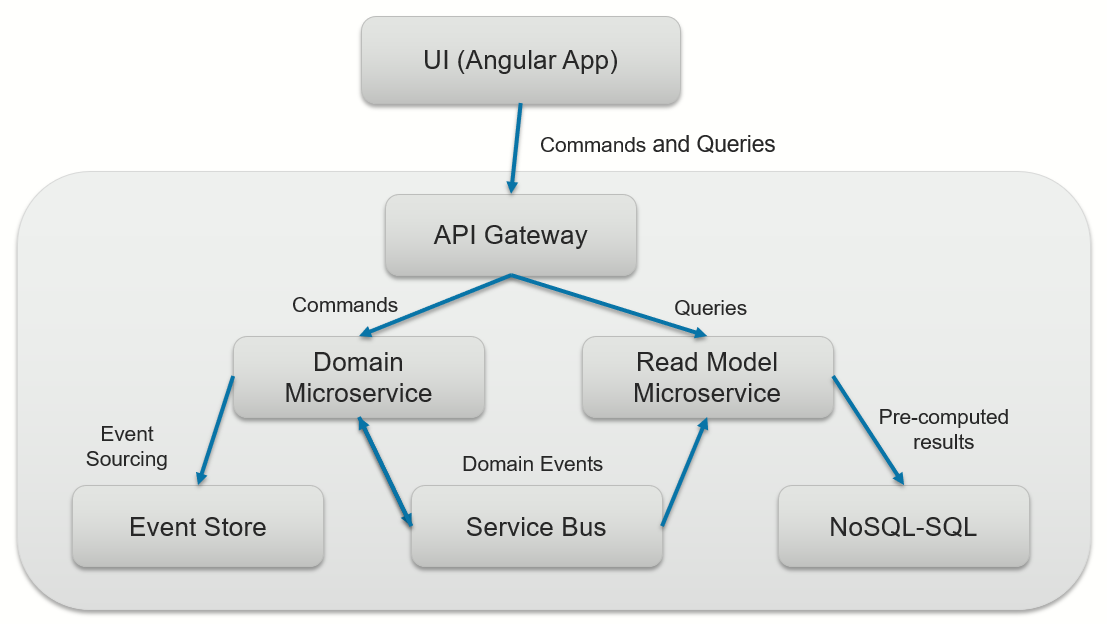
\includegraphics[width=10cm]{algArch.png}
	\centering
	\caption{Een algemene architectuur voor microservices. \textcite{Koukia2018}}
\end{figure}
Als eerste wordt er een request gemaakt. Die wordt naar de gateway gestuurd. Dan wordt er gekeken, moet er een commando of een query uitgevoerd worden. Bij een commando wordt er naar een domein microservice gestuurd en anders naar een real-model microservice.  Daarna worden er gegevens opgeslaan.


\subsection{Het belang van microservices}
Bij een monolithic kan het aanpassen van een deeltje, veel werk vragen. Dit werd meer uitgelegd bij de definite van microservices. Microservices spelen gemakkelijker in op het periodieke opleveren van delen software. Deze technologie legt niet heel het framework plat als er deeltjes moeten bij gecodeerd worden. Microservices kunnen sneller inspelen op de Agile analyse/ontwikkel methode. Dit is ook een reden waarom microservices zo een opkomst kent. De analyse methode Agile werkt met periodieke opleveringen die kunnen gaan van twee weken tot een maand. In de periode wordt er gewerkt aan een functionaliteit of een eis van de klant. 
Er voor zorgen dat software schaalbaar is, is een belangrijk punt en daar spelen microservices goed op in, \textcite{series2018}.



\textcite{Troisi2019} geeft acht best practices over de bescherming van microservices. 
De best practices:
\begin{itemize}
	\item Het gebruik van OAuth voor gebruikers identificatie en wat de gebruiker kan. OAuth/OAuth2 is een protocol voor authorisatie. Het is een gemak om gebruik te maken van een protocol. Een protocol zijn een aantal regels om te communiceren tussen computers. 
	\item Gebruik bescherming in de diepte om een prioriteit toe te kennen aan service keys.  Dit kan verwoord worden als bescherming steken in verschillende lagen van een systeem. Er moet worden nagegaan welke deeltjes het kwetsbaarst zijn en daar dan op verschillende lagen van beveiliging op toepassen. 
	Microservices maken het toepassen van deze methode, eenvoudiger. Doordat er gefocust kan worden op beveiliging. Het framework maakt het gemakkelijker om de verschillende lagen vast te stellen. Als ze binnen zijn bij een van de microservices zijn ze niet binnen in het volledige systeem. 
	\item Schrijf zelf geen krypto code. Er zijn genoeg open source alternatieven. Enkel bij heel uitzonderlijke redenen wordt een eigen crypot code geschreven. 
	\item Update je bescherming tijdig. Als er updates komen in de software van beveiliging, moeten die ook uitgevoerd worden. Het automatiseren van die updates, kan veel werk besparen achteraf. Dit wordt dan ook best gedaan bij het begin van microservices. Bescherming binnen software is niet meer een nice to have maar een must have. 
	\item Maak gebruik van een firewaal met gecentraliseerde controle. Het biedt ook meer controle aan aan de gebruiker.
	\item Zorg dat je 'containers' niet in een publiek netwerk te vinden is. Dit is eigenlijk zorgen dat gebruikers je achterliggende architectuuur niet kunnen zien. Ervoor zorgen dat erna maat één toegangspoort is.  Hier kan een vorige manier ook bijgestoken worden. Microservices kunnen achter een firewall gestoken worden als bescherming.  Als er met containers wordt gewerkt, moet er ook beschemring aanwezig zijn. Een container is een plek waar kleine deeltjes code kunnen op gedeployed worden. 
	\item Maak gebruik van software om virussen te vinden.
	\item Monitor alles.
\end{itemize}

Nog andere redenen om microservices te gebruiken, \textcite{Koukia2018}, zijn volgende:
\begin{itemize}
	\item Het is gemakkelijker om kleine services te onderhouden. Bij een monolithic is alles één groot geheel, als daar een deeltje van moet worden uitgelegd, kan je verdwalen in het grote geheel. Dit is niet zo bij microservices. Want elke services is afgebakend met een functionaliteit. Bij het uitleggen van een services kan er duidelijk aangetoond worden waar een services begint en eindigt. 
	\item Een microservices kan onafhankelijk gedeployed worden. Eens een microservices klaar is om gebruikt te worden, moet er naar niks anders gekeken worden. Bij het deeltje definitie werd hier dieper op ingegaan.
	\item Gemakkelijker aan te passen aan nieuwe technologie. Komt er een nieuwe technologie uit die kan toegepast worden op een paar microservices, dan moeten enkel die microservices herschrijven worden. Dit ligt in contrast met een monolithic. Als er een nieuwe technologie is die kan toegepast worden op onderdelen van het geheel, moet de gehele architectuur herschreven worden.
	\item Het is eenvoudiger om te scalen. Zoals al eerder aangehaald, kan schalen van de architectuur gebeuren door de microservices te dupliceren. Niet het gehele systeem moet geschaald worden, enkel de nodige microservices moeten gedupliceerd worden. 
	\item No single point of failure. Faalt er een microservices in het uitvoeren van zijn functionaliteit, dan heeft dit geen invloed op de andere services. Hier is dieper op ingegaan tijdens de definitie.
	\item Freedom of technology stack choices. Dit omvat dat elk team kan kiezen in welke programmeertaal ze de microservices schrijven. Een team is verantwoordelijk voor één microservices. Ze zijn dus gespecialiseerd in die ene service. 
	\item De evolutie en de oplevering van business features is sneller. Dit komt door de onafhankelijkheid van de services. Er kan op het zelfde moment aan verschillende services gewerkt worden, zonder elkaar te beïnvloeden.
\end{itemize}


Onder volgende deeltjes wordt er dieper ingegaan op de authenticatie en authorisatie, het verband met Agile en Devops, het debuggen binnen microservices en de bescherming van microservices.

\subsubsection{De verschillende manieren van bescherming}
Microservices moeten een doel in de business vervullen. Naast dit, zorgen microservices er ook voor dat de bescherming eenvoudiger wordt, \textcite{RDX2016}.

Enkele tips om de bescherming van microservices aan te pakken, \textcite{Matteson2017}, \textcite{Silva2017}:
\begin{itemize}
	\item Zorg bij het ontwikkelen van microservices voor coderingsstandaarden die kunnen herbruikt worden. Door eenmaal een goede code te voorzien wordt de kans op kwetsbaarheden en gaten in de bescherming kleiner.
	\item Ga na welke schade er kan toegebracht worden aan een microservice als die zonder bescherming zou worden geupload.
	\item Maak gebruik van toegangscontroles. Zorg ervoor dat er gewerkt wordt met leesrechten. Een microservice dat de aankooporders ophaalt moet niet aan de verkooporders kunnen.
	\item Ga geen beveiligingsprincipes gebruiken van externen, implementeer die in de code van de microservice.
	\item Zorg voor goede documentatie van elke microservice. Dit kan handig zijn bij het ontdekken van een zwak punt in de bescherming. De documentatie kan mogelijke problemen verduidelijken.
	\item Maak een API gateway. Wat het precies allemaal doet wordt verder nog uitgelegd.
	\item Zorg ervoor dat enkel de API gateway zichtbaar is en dat alle data onleesbaar moet worden verzonden. Dit kan gebueren aan de hand van SSL of TSL. Wat SSL is wordt verder in deze thesis uitgelegd. 
	\item Zorg voor garantie op data privacy. In Europa is de GDPR een wetgeving die zegt wat er wel en niet mag gebeuren met mensen hun data. Daarom is het belangrijk dat er gebruik wordt gemaakt HTTPS. Op elk level moet er gezorgd worden voor een correcte beveiliging van de gebruikers hun data. 
	\item Voor het encrypteren van data, wordt er best gebruik gemaakt van al bestaande technologies. 
	\item Zorg ervoor dat er geen denial of service kan gebeuren. Denail of service komt voor wanneer er heel veel requests naar de applicatie worden gestuurd, waardoor de applicatie faalt. Maak gebruik van throtteling. De term wordt na deze opsomming verder uitgelegd.
	\item Maak gebruik van CSRF en CORS filters. Cross-site request forgery is een poging tot hacken waarbij de eindgebruiker gedwongen wordt om acties te doen terwijl hij geauthenticeerd is. Cross-origin resource sharing laat toe dat er requests van een ander domein kunnen worden gemaakt. 
	\item De API gateway mag nog zo goed beschermd zijn als iets, zorg ook voor goede bescherming aan de code. Zorg ervoor dat er niks moet worden gerund als administrator, geef duidelijke namen. Zorg ervoor dat enkel de nodige personen de juiste permissies krijgen. 
\end{itemize}

Throtteling, \textcite{Cavalcanti2018}, is een manier van bescherming die het volgende inhoud: "Throttling is a process used to control the usage of APIs by consumers during a given period.". Het kan zijn dat de gebruiker heel veel requests stuurt naar de API gateway of een bug kan zorgen voor een oneidig aantal request. Om dit te voorkomen kan er een limiet aantal request  binnen een bepaalde periode opgelegd worden. Bijvoorbeeld als je je toegangscode drie maal fout hebt op je gsm, dan blokeert die voor een bepaalde tijd. Het systeem zo ontwerpen dat het bestand is tegen fouten en falen. Met bestand zijn tegen, wordt bedoelt om ervoor te zorgen dat bij een bug of een fout, deze goed wordt opgevangen zodat de gebruiker er geen last van heeft. 

Eén van de meer bekendere manieren is, API gateway. De verantwoordelijkheden van een API gateway zijn volgende, \textcite{Siraj2017}:
\begin{itemize}
	\item Het ontvangen van request van gebruikers.
	\item De requests doorsturen naar de correcte microservice.
	\item Het 'antwoord' van de microservice in ontvangst nemen en doorsturen naar de gebruiker.
\end{itemize}
Zoals te zien is op figuur X, is een API gateway het toegangspunt. API gateway wordt gebruikt voor authenticatie en authorisatie. Meer uitleg hierover in de sectie over authenticatie en authorisatie.
\begin{figure}[h]
	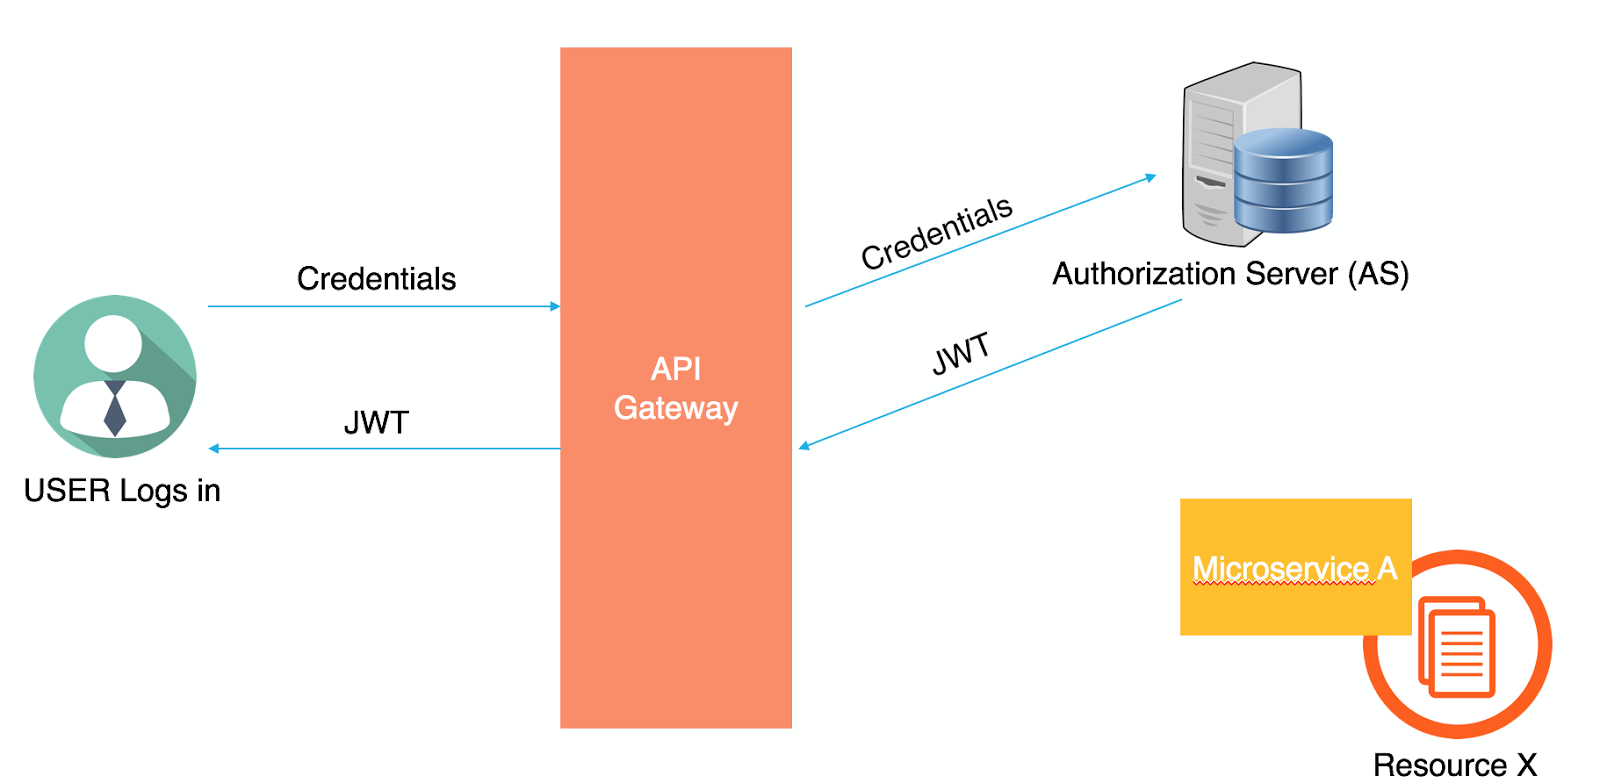
\includegraphics[width=10cm]{apiGateway_facadePattern.png}
	\centering
	\caption{Een voorstelling van API gateway. \textcite{Siraj2017}}
\end{figure}


\subsubsection{Authenticatie en authorisatie}
Een belangrijk aspect van microservices is de authenticatie en de authorisatie.  Het is een moeilijkheid om op een uniforme manier veiligheid, bescherming, authorisatie en authenticatie toe te passen op microservices, \textcite{Ayoub2018}. Authenticatie is bevestigen dat jij het bent. Dit wordt gedaan via een gebruikersnaam en een wachtwoord. Authorisatie is wat je kan doen met een programma. Bijvoorbeeld een beheerder van een site kan meer dan een bezoeker. 
\begin{figure}[h]
	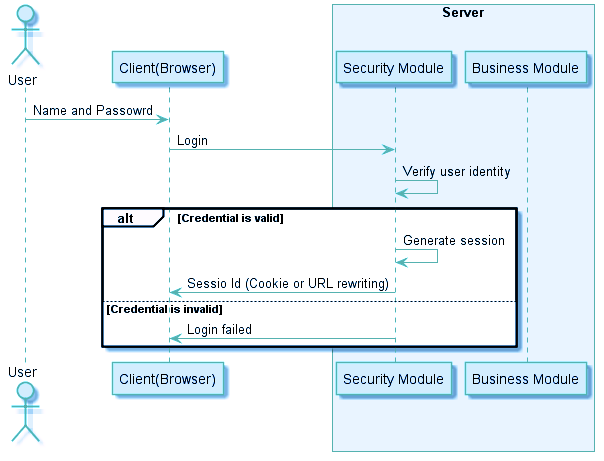
\includegraphics[width=10cm]{monolithic_auth.png}
	\centering
	\caption{Een diagram van authenticatie bij een monolithic. \textcite{Ayoub2018}}
\end{figure}
Zoals te zien is op bovenstaande afbeelding, figuur 2.3, wordt de authenticatie afgehandeld binnen het monlithic proces. Wanneer de gebruiker inlogt, wordt de beveiligings module aangesproken. Deze kijkt of de gebruiker een bekende is, of er al gegevens in de databank zitten. Als het aanmelden gelukt is, wordt er een sessie gecreëerd. Een sessie wordt opgeslaan aan de hand van cookies. Cookies worden op je computer geplaatst door je browser. Het zijn kleine tekstbestanden. De sessie onthoudt wie je bent aan de hand van een ID. Dit zorgt ervoor dat je je niet elke keer opnieuw moet aanmelden als je van pagina verandert.  Elke keer dat de bezoeker van de site iets doet, wordt de sessie ID samen gestuurd met de request. Een request is een aanvraag. Als het ID correct is, weet de site dat de gebruiker ingelogd is. Bij elke aanvraag wordt de ID meegestuurd zodat er kan gecontroleerd worden of die zo wordt de authenticatie bij een monolithic afgehandeld.
Wanneer er gekeken wordt om authenticatie toe te passen bij microservices, komen volgende puntjes veel voor:
\begin{itemize}
	\item In elke microcservice moet er authenticatie en authorisatie afgehandeld worden. Het beste wordt dit toegepast op een uniforme manier. Dan wordt er van uit gegaan dat er in elke microservices een stukje code gaat komen dat herbruikt wordt. Maar dit zorgt ervoor dat elke microservice toch afhankelijk is. Bij het uitkomen van een nieuwe versie, moet dit deeltje dan weer geüpdate worden. Dit heeft invloed op de flexibiliteit van het framework.
	\item "Single responsibility" zijn twee woorden die microservices mooi omschrijven. Een microservice omvat een stukje business logica. De algemene logica van authenticatie en authorisatie mag niet in een microservices gegoten worden. 
\end{itemize}
In het algemeen zijn authenticatie en authorisatie een complex onderdeel van microservices.
Er zijn vijf oplossingen volgens dit artikel.
\begin{itemize}
	\item Distributed session manangement,
	\item client token,
	\item single sing-on, 
	\item client token with API gateway.
\end{itemize}
Distributed Session management is de eerste oplossing. Het managen van een sessie over microservices. Dit kan op verschillende manieren. Aan de hand van Sticky sessions. Dit houdt in dat alle requests van één gebruiker naar dezelfde server worden gestuurd. Dan kan men ervan uitgaan dat de gebruikte data van die specifieke gebruiker is. Of men kan dit toepassen via session replication. Dit houdt in dat alle instanties de sessie data synchronizeren. Deze manier van toepassen heeft als nadeel dat er veel overhead zal zijn op het netwerk. Een andere methode is centralized session storage. Dit omvat dat bij het aanspreken van een microservice, deze de gebruikers data gaat ophalen van op een gedeelde plaats. 
Een andere manier om authenticatie en authorizatie toe te passen is via een client token. Een token wordt gebruikt om aan te tonen dat je ook echt de gebruiker bent. Een token wordt bijna altijd onleesbaar gemaakt. Het klinkt bijna hetzelfde als een sessie. Het verschil ligt hem in het feit dat een sessie op de server centraal wordt bijgehouden. Een token wordt bijgehouden door de user zelf.
Naast de Distributed session management en client token is er ook nog single sign-on. Na een enkele aanmelding, kan de gebruiker alle microservices gebruiken binnen de applicatie. 
Een andere manier is een client token wiht API gateway. Deze manier is gebaseerd op de client token. Maar nu is er een API gateway toegevoegd aan het begin van een externe request. Dit zorgt ervoor dat het framework niet zichtbaar is aan de buitenwereld. 

\begin{table}[]
	\resizebox{\textwidth}{!}{%
		\begin{tabular}{|p{3cm}|p{10cm}|p{10cm}|p{10cm}|}
			\hline 
			Eigenschappen 
				& Sidecar proxy 
				& API gateway
				& Single SignON (SSO) \\ \hline
			Wat?  
				& "A sidecar proxy, is a proxy running in the same host where your microservice is deployed", \textcite{Cavalcanti2018}.
				& "An API gateway is a piece of software running on or near the periphery of the network hosting your system services", \textcite{Everard2017}. 
				& "SSO simply means login, just once to a suite of independent applications.", \textcite{Everard2017}. \\ \hline
			Heeft volgende opties:
				& De ingebouwde functies zijn volgende:
					\begin{itemize}
						\item Authenticatie/authorizatie
						\item Retry policies
						\item Routing
						\item Error afhandeling
						\item circuit-breakers: Een automatische machine voor het stoppen van de flow voor veiligheidsredenen.
					\end{itemize} 
				& / 
				& Bij het inloggen wordt een cookie aangemaakt die dan wordt opgeslaan in de API gateway. \\ \hline
			Voordelen 
				& De niet-functionele onderdelen van de microservice(s) kunnen hieronder gebracht worden. 
				& Dit zorgt ervoor dat de microservice zich enkel moet bezig houden met de business logica.
				&  \\ \hline
			Nadelen
				& Er komen meerdere componenten bij om te monitoren, te onderhouden en te deployen. 
				& Omdat dit een single point of entry kan dit een bottleneck, een plek van opstopping, zijn in de architectuur. 
				& \\ \hline
			
		\end{tabular}%
	}
	\caption{De verschillende manieren voor authenticatie en authorisatie toe te passen.
		\textcite{Cavalcanti2018}, \textcite{Everard2017} }
\end{table}

De meest voorkomende methodes in API authenticatie terug te vinden in tabel X, \textcite{Sandoval2018}.
\begin{table}[]
	\resizebox{\textwidth}{!}{%
		\begin{tabular}{|p{2cm}|p{10cm}|p{10cm}|p{10cm}|}
			\hline 
			 
				& HTTP Basic Authentication
				& API keys
				& OAuth \\ \hline
			Definitie  
				& "A HTTP user agent simply provides a username and password to prove their authentication". 
				& "An unique generated value is assigned to each first time user, signifying that the user is known. When the user attempts to re-enter the system, their unique key is used to prove that they’re the same user as before.".
				& "The user logs into a system. That system will then request authentication, usually in the form of a token. The user will then forward this request to an authentication server, which will either reject or allow this authentication. From here, the token is provided to the user, and then to the requester. Such a token can then be checked at any time independently of the user by the requester for validation, and can be used over time with strictly limited scope and age of validity".\\ \hline
			Voordelen
				& Er is geen nood aan cookies, session ID's, login pagina's, ook een handshake bevestigen is niet nodig.
				& Dit is een manier van authenticatie die snel gebeurt. Het is een niet zo complex proces om de sleutels te genereren. 
				& Het is de beste manier van authenticatie en authorisatie uit deze tabel. \\ \hline
			Nadelen
				& Is er geen SSL (Secure Sockets Layer) aanwezig dan is het eenvoudig om de gegevens op te halen en ligt alles open en bloot op het internet. Ook bij het gebruik van SSL is er een nadeel. De tijd dat moet gewacht worden op een antwoord wordt vertraagd.
				& De API key is niet geschikt voor authorisatie. Bij het fout gebruik van API keys kan dit een grote impact hebben op de bescherming van de applicatie.
				& Als er enkel gebruik moet gemaakt worden van één van de twee, authenticatie of authorisatie, dan is OAuth overbodig. Want OAuth heeft veel meer te bieden. 
				\\ \hline
		\end{tabular}%
	}
	\caption{De verschillende methoden in API authenticatie, \textcite{Sandoval2018}}
\end{table}

Het proces van een API gateway dat authenticatie en authorisatie op zich neemt, \textcite{Siraj2017}.
Door de API Gateway to combineren met JSON Web Tokens is er meer mogelijkheid om te schalen. 
\begin{enumerate}
	\item De gebruiker meldt zich aan.
	\item De API gateway stuurt de request door naar de server die instaat voor de auhtenticatie.
	\item is de authenticatie goedgekeurd, wordt er een JWT token terug gestuurd naar de gebruiker. Meer uitleg over de JWT na dit proces.
	\item Bij volgende request wordt de token automatisch meegestuurd met de request.
	\item Een andere server kijkt bij elke request naar de token, om na te gaan of de gebruiker de juiste authorisatie heeft. 
\end{enumerate}
De token vervalt na een bepaalde tijd. Er kan gekozen worden om deze automatisch te laten verlengen. Hier wordt niet verder op ingegaan. 

De definitie van JSON Web Token, \textcite{Stecky-Efantis2016}: "A JSON Web Token (JWT) is a JSON object that is defined in RFC 7519 as a safe way to represent a set of information between two parties. The token is composed of a header, a payload, and a signature.". Het diagram te zien in figuur X, is een schematische voorstelling van hoe een JWT token wordt gegeven aan een gebruiker.
\begin{figure}[h]
	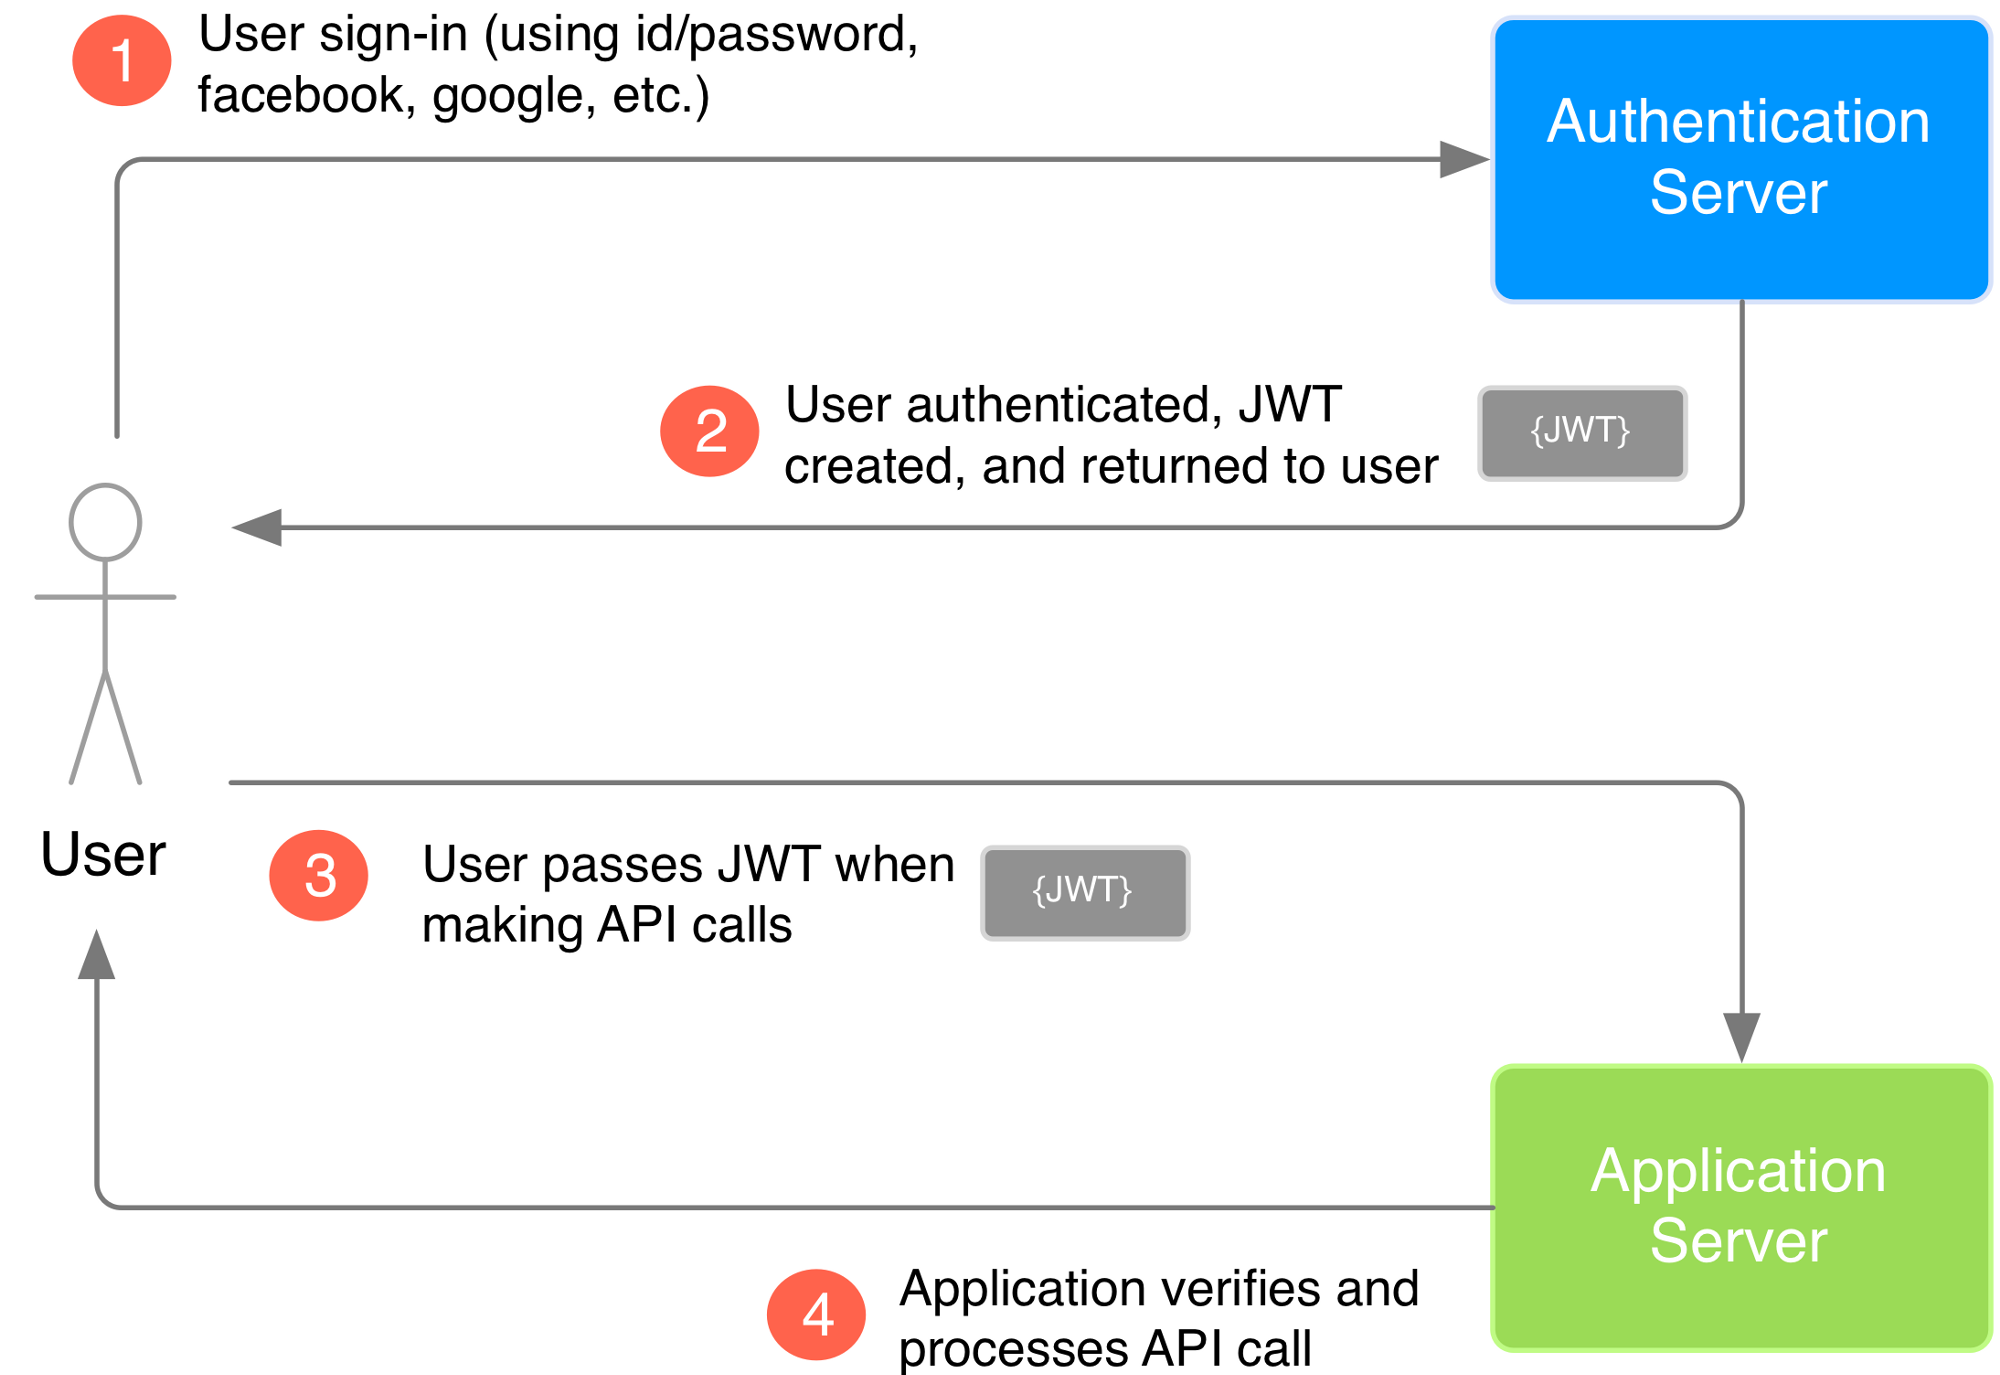
\includegraphics[width=10cm]{jwt.png}
	\centering
	\caption{Een schematische voorstelling van het geven van een JSON Web Token. \textcite{Stecky-Efantis2016}}
\end{figure}
Het proces gaat als volgt:
\begin{enumerate}
	\item Aanmelden op een platform. Bijvoorbeeld aanmelden op facebook, twitter, instagram of google.
	\item De authenticatie server stuurt een JWT terug.
	\item Bij het maken van requests wordt de token meegestuurd.
	\item De microservice kijkt dan of de gebruiker het recht heeft om deze microserivce/functie te gebruiken.
\end{enumerate}


\subsubsection{Verband met Agile en DevOps}
Microservices komen uit dezelfde ideologie als Agile en DevOps. DevOps is een samenvoegsel van development en operations. Bij deze methode ligt de nadruk op de samenwerking en communicatie tussen verschillende partijen. Hier zijn de partijen de software engineers en andere IT specialisten. Deze ideologie omvat het volgende: het afbreken van kleine, traag evoluerende architectuur of monolithic en deze in microservices steken.

DevOps heeft volgende definitie: "DevOps is a methodology that enables developers and IT Ops to work closer together so they can deliver better quality software faster", \textcite{Morgan2019}. Met DevOps probeert de productie zo goed mogelijk na te bootsen. Net zoals bij Agile, zorgt DevOps ervoor dat de software in kleinere delen wordt opgesplitst om ook weer op kortere periodes kleinere deeltjes software op te leveren. Dit is iets waar ook microservices in terug te vinden is. Verschillende DevOp teams kunnen dus tegelijkertijd werken aan microservices werken.

Enkele voordelen van de combinatie microservices en DevOps:
\begin{itemize}
	\item Meer opleveringen van software op kortere periodes.
	\item Betere kwaliteit van de code.
	\item Software kan hergebruikt worden.
	\item Een hoger level van automatisatie.
\end{itemize}

Microservices en DevOps vullen elkaar aan op volgende vlakken, \textcite{Mulesoft2019}:
\begin{itemize}
	\item Deployability: Microservices bemoedigen het gebruik van Agile omdat het eenvoudiger is om periodiek op te leveren. 
	\item Reliability: Een fout binnen een microservice, heeft enkel effect op die microservice. 
	\item Availability: Het opleveren van nieuwe deeltjes, neemt niet veel tijd in beslag. De gehele applicatie zal niet lang offline zijn.
\end{itemize}




\subsubsection{Het monitoren van microservices}
Logs zijn records binnen een databank waar naar weggeschreven wordt terwijl de applicatie draait. Metrics zijn numerieke waarden die kunnen geanalyseerd worden. Metrics zijn terug te vinden op volgende niveau's van een applicatie, \textcite{Wasson2018}:
\begin{itemize}
	\item Node-level: Dit houdt in de gegevens van de CPU, het geheugen, netwerk en de harde schijf. 
	\item Container: Draait de service binnen een container dan moeten er ook metrics bijgehouden worden van die container. 
	\item Applicatie: Hier kunnen metrics bijgehouden worden om het gedrag van de service te begrijpen. Gegevens die kunnen bijgehouden worden zijn het aantal HTTP requests, de vertraging en de lengte van een bericht.
	\item Dependent service: Bij interactie met een externe service, hoelang deze duurt voordat de externe service reageert. 
\end{itemize}


Het monitoren of loggen van microservices houdt in dat er wordt bijgehouden hoe een microservice zich gedraagt. Er wordt bijgehouden hoe snel de data wordt opgehaald uit de databank. Ook voor het vinden van problemen is monitoren een belangrijk onderdeel. Dankzij monitoring kan een fout sneller gevonden worden. Er kan worden nagegaan hoelang het duurde om een bepaalde request te maken. Van die gegevens kunnen er dan conclusies getrokken worden, \textcite{Ananthasubramanian2018}.

Loggen is belangrijk omdat bij meedere services het moeilijk kan zijn om het traject binnen de services te volgen, \textcite{Saldanha2016}.

De verschillende tools om te debuggen, \textcite{Swersky2019}:
\begin{itemize}
	\item Logging frameworks: Het is een open-source oplossing. Er zijn verschillende opties, bij het kiezen wordt er best rekening gehouden met volgende puntjes:
		\begin{itemize}
			\item De netheid van de code. Is de logging code gemakkelijk te lezen?
			\item Wordt de performance beeïnvloedt?
			\item Is het framework voor logging al gekend onder het team?
		\end{itemize}
	\item Logging databases: Log data wordt gebruikt voor het captueren van events. Logs worden nooit aangepast. Logs worden ook gesorteerd op datum en tijd. 
\end{itemize}



Bij microservices wordt elke microservice gelogd. Bij een fout moet er gekeken worden naar alle betrokken microservices. Er moet gekeken worden naar alle logs van de services. Om logging toe te passen wordt er aangeraden om libraries te gebruiken. Enkele best practices, \textcite{Melendez2018}, \textcite{Eyee2018}, \textcite{Timms2018}:
\begin{itemize}
	\item Probeer te vermijden dat logs in bestanden worden opgeslaan. Logs zijn streams van een flow. Het geeft weer wat er juist gebeurt is in een flow.
	\item Microservices moeten niet weten waar de logs naartoe gaan. Zo kan de bestemming van het wegschrijven van de logs veranderd worden zonder dat elke microservice ervoor moet aangepast worden.
	\item De logging zou moeten werken voor alle verschillende codeertalen. Er zou niets moeten worden aangepast bij de configuratie files van het logging systeem.
	\item Geef elke request een uniek ID. Zo kan de request snel teruggevonden worden bij falen. Of bij het zien van een fout kan er snel achterhaald worden welke request er in fout is gegaan. 
	\item Laat het antwoord ook een uniek ID meesturen. Als de gebruiker dan een fout krijgt, kan er achterhaald worden vanwaar de teruggestuurde fout komt. De administrators kunnen dan de details van de fout bekijken.
	\item Een oplossing is om alle logs weg te schrijven naar een centrale databank. Zo kan het hele pad van de fout snel en eenvoudig teruggevonden worden. Het duurt langer om verschillende fouten aan elkaar te linken als de logs in de datastore van de microservice worden opgeslaan. Bij het opslaan op één plaats, worden fouten sneller aan elkaar gelinkt. Het wegschrijven naar een plaats is tegen het principe van microservices. Elke microservice op zichzelf. Binnen die enkele database met alle logs kan er gezocht worden op fout, microservice, tijdstip, .... Ook het volgen van een gebruiker zijn traject binnen de applicatie is eenvoudiger. Bij een fout kan er gekeken worden naar de acties die er op voorhand zijn gemaakt. 
	\item Zorg voor structuur in de log data. Een algemene format zoals JSON of XML om een structuur te steken in je logs. 
	\item Geef elke request een context. Weten wat gezorgt heeft voor de fout, is belangrijk om ervoor te zorgen dat de fout niet nog eens voorkomt. Volgende velden zouden zeker in de log terug te moeten vinden zijn:
		\begin{itemize}
			\item Dag en tijd.
			\item Stack errors.
			\item De naam van de service, om de logs te linken aan microservices.
			\item In welke functie de fout is ontstaan.
			\item De naam van de externe service waar er interactie mee is geweest.
			\item Het IP adres van de server en van de gebruiker zijn requests. 
			\item De browser waaruit de gebruiker de request stuurde.
			\item De HTTP code om later alerts te creëren. 
		\end{itemize}
	\item Overweeg om de logs naar een lokale databank weg te schrijven. Elke oplossing heeft zijn voordelen en nadelen. Het wegschrijven over HTTP naar de cloud kan zorgen voor meer verkeer op het netwerk. Dus er kan bandbreedte weggenomen worden van belangrijkere microservices. 
	\item Kijk na wat er gelogd wordt, is het niet nodig om iets te loggen, laat het achterwege. Maar bij de start van loggen, wordt er best te veel gelogd. Zodat er eerst teveel info is en dan kan er gesneden worden in de inhoud van het loggen.
\end{itemize}



\subsection{Algemene aanpak om microservices te implementeren}
Voordat er wordt begonnen aan het overschakelen naar microservices, moet er research gedaan worden, \textcite{Koukia2018}. De logische eerste stap is het lezen van artikels en hoe andere bedrijven zijn overgeschakeld naar microservices. Wat hun problemen en moeilijkheden waren. Door artikels en ervaringen van anderen te lezen, kan je zelf mogelijke problemen voorkomen. Na de verdieping in microservices, moet er een plan opgemaakt worden. Dit plan wordt best met meerdere mensen samen gemaakt. Zodat er meer mensen kunnen nadenken en om ervoor te zorgen dat iedereen op dezelfde lijn zit.


\textcite{Benetis2016} schreef een 6-stappen plan om microservices te implementeren. Over de grote lijn wordt er daarop gebaseerd, maar per stap gaat er dieper op worden ingegaan.
Een paar woorden die meer verklaring nodig hebben voordat we verder gaan. Een gateway is een netwerkpunt dat dient als toegang tot een ander netwerk. Een gateway is een soort toegangspoort. 
Implementatie is een procesmatige invoering van een verandering of vernieuwing. Iets implementeren of vernieuwen. 

In grote lijnen is dit het zes-stappen plan. Als eerste komt aan bod "serve a business purpose". Hierna komt "protect your stuff". Eens dat gebeurt is, zegt het artikel "see no evil, hear no evil". Dan komt "find your stuff" aan bod. Hierna wordt de volgende stap "create a gateway" aangehaald. Als laatste komt "construct events" aan de beurt.

De eerste stap is "Serve a business purpose". De titel zegt al veel van wat er verwacht wordt. Een microservices is gebaseerd op een business requirement. En niet het doel dat het IT-team voor ogen heeft. Een voorbeeld van een business requirement is het ophalen van data om die dan te analyseren om daar later dan conclusies uit te trekken. Dit kan in een microservices gegoten worden. Eens het doel voor ogen is bij een microservices, moet er ook gekeken worden naar wat de microservices moet kunnen. Zo lang het bij enkele microservices blijft, is automated deployement etc. niet zo belangrijk. Maar eens we gaan scalen en meerdere microservices in één systeem steken zouden volgende puntjes toch self-sufficient moeten zijn:
\begin{itemize}
	\item Geautomatiseerde implementatie
	\item Blootstelling aan andere systemen, toegankelijk eindpunt
	\item Opslag van data
	\item Schaalbaarheid en belasting
\end{itemize}
Zoals te zien is op figuur 2.2, is een microservices één klein deeltje in een groot geheel. Later in dit stappenplan zal de figuur ook uitgebreidt worden en zal het geheel duidelijk worden. 
\begin{figure}[h]
	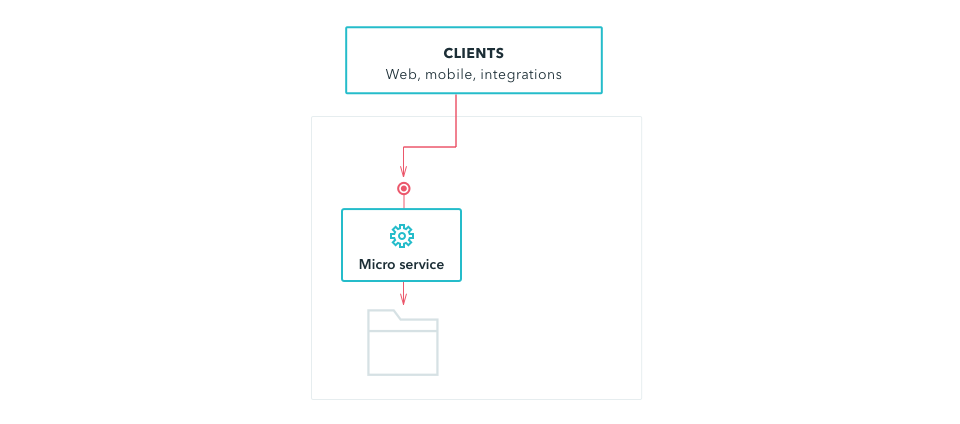
\includegraphics[width=10cm]{1.png}
	\caption{Een microservice dat voldoet aan een business requirement. \textcite{Benetis2016}}
	\centering
\end{figure}

Na "Serve a business purpose" komt "Protect your stuff". Dit gaat over de bescherming van een microservices. Als het gaat over bescherming moet dit op elk moment gebeuren. Ookal heb je maar één à twee microservices, of honderden, bescherming is belangrijk. Het is belangrijk op over al de microservices een uniforme manier te vinden om ze te beschermen. De bescherming kan een requirement op zich zijn, dus ook dit kan in een microservices worden gestoken. Bescherming is een vage term daarom een korte uitleg van hoe een bescherming er zou kunnen uitzien. De meest bekende manier is natuurlijk authorisatie en authenticatie. Authorisatie is het verkrijgen van rechten om bijvoorbeeld een product toe te voegen op een site. Authenticatie is het aanmelden op facebook bijvoorbeeld. De controle of jij het wel echt bent. Een manier op de microservices te beschermen is gecentraliseerde session opslag. Hier zal verder in de thesis nog dieper op worden ingegaan. Kort uitgelegd betekend gecnetraliseerde session opslag dat de data van de user centraal opgeslagen staat. Zodat alle microservices de zelfde session data lezen en gebruiken. 
\begin{figure}[h]
	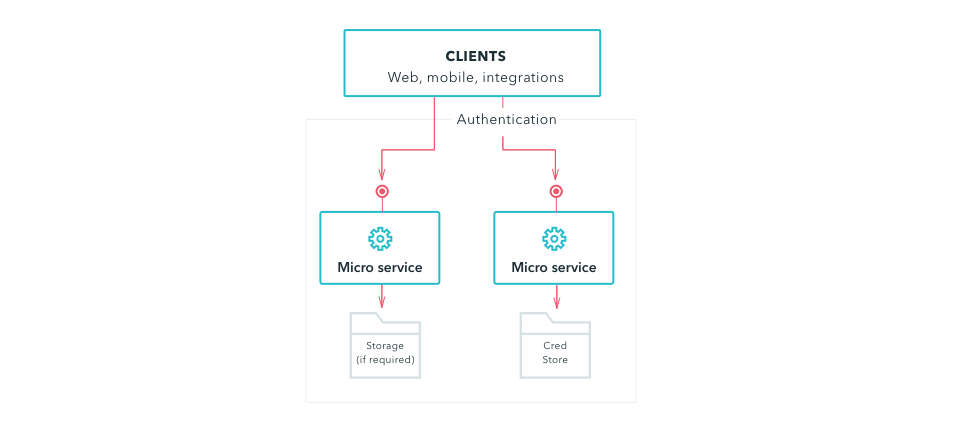
\includegraphics[width=10cm]{2.png}
	\caption{Een microservice waar bescherming aan is toegevoegd. \textcite{Benetis2016}}
	\centering
\end{figure}
In figuur 2.3 is de authenticatie in een microservices gestoken. 

Na de eerste twee stappen komt "See no evil, hear no evil". Eens de microservice is opgezet en gedeployed, moet er gemonitord worden. Daarmee wordt bedoeld dat hoe de microserivces zich gedraagd goed moet bijgehouden worden. Alles zou goed moeten gelogd worden, zodat bij een probleem het geen moeite is om te vinden waar het probleem zich voordeed. Ook hier is het aangeraden om doorheen het hele systeem een uniforme manier van loggen aan te houden. Ook kan men hiervan een microservice maken. Dit wordt ook afgebeeld in figuur 2.4.
\begin{figure}[h]
	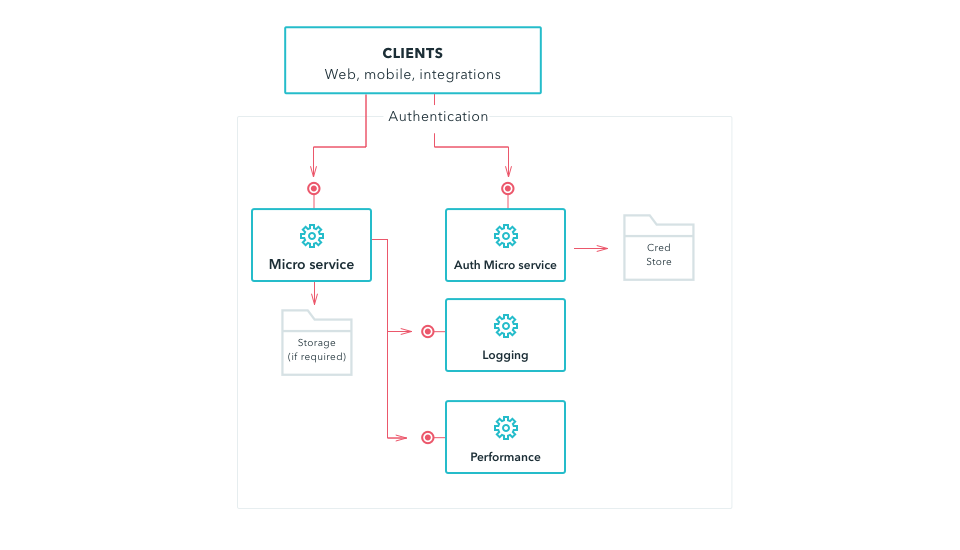
\includegraphics[width=10cm]{3.png}
	\caption{Een microservice waar er monitoring is aan toegevoegd om chaos te voorkomen. \textcite{Benetis2016}}
	\centering
\end{figure}

Als vierde stap komt er "Find your stuff". In deze stap wordt er gezocht naar een manier om de microservices met elkaar te communiceren. Hiermee wordt bedoelt hoe dat microservices A gegevens vraag aan microservices B. Die dat dan ook vraagt van een andere microservice. Een veel gebruikte techniek hiervoor is "service registry". Een service registry is een databank waar alle services met hun instanties en locatie woren opgeslaan. Daar worden dan ook connecties in opgeslaan. Ook hier wordt er aangeraden om dat in een microservices te gieten. Zodat ook hiervan het gedrag kan gemonitord worden. In figuur 2.5 zie je hoe de service registry kan toegevoegd worden. In de figuur is die terug te vinden onder de naam "service discorvery".
\begin{figure}[h]
	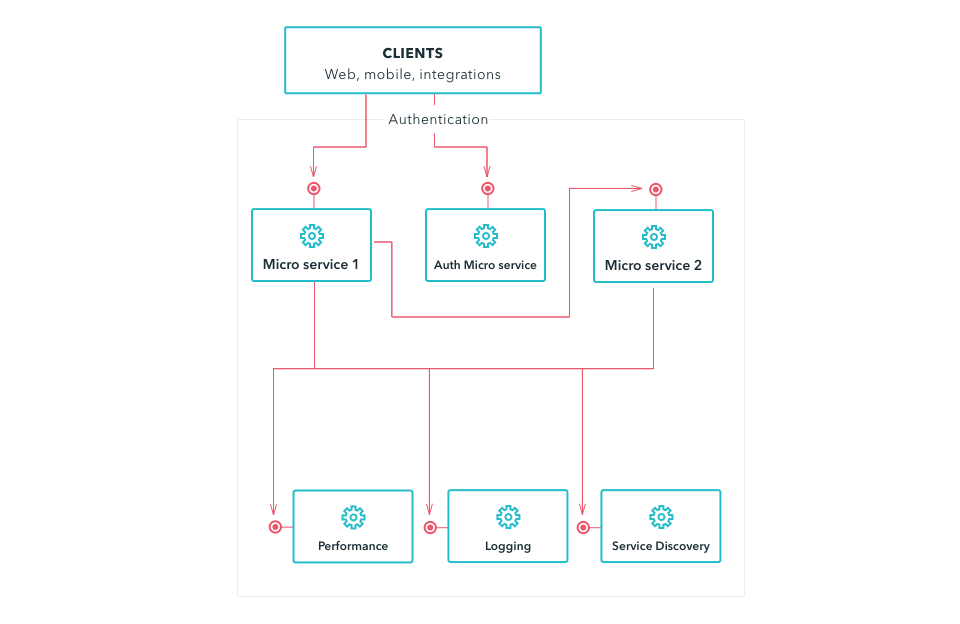
\includegraphics[width=10cm]{4.png}
	\caption{Een microservice dat authenticatie als bescherming toepast. \textcite{Benetis2016}}
	\centering
\end{figure}

Nu is er een service, bestaande uit microservices, dat beschermd is en kan doen wat het zou moeten doen. Maar niet de  volledige service moet open en bloot gelegd worden. En daar zorgt stap 5, "Create a gateway", voor. Een API gateway kan een scherm zijn waar je gegevens op invult en mogelijke acties op doet en die spreken dan de correcte microservices aan. De taak van een gateway is voornamelijk zorgen dat request/aanvragen naar de juiste microservice worden doorgestuurd. Andere taken van een API gateway kunnen volgende zijn
\begin{itemize}
	\item Beveiliging: een API gateway kan de binnenkomende aanvragen valideren. 
	\item Prestatiegegevens kunnen geregistreerd worden.
	\item Omzetten van aanvragen in enkele of meerdere microservices.
	\item Abstractie van de clientinterface. Wanneer er van microservice verandert wordt, moet er niet van interface/scherm verandert worden. 
\end{itemize}

In figuur 2.6 is te zien hoe zo een API gateway kan worden toegepast. Zo is ok te zien dat de authenticatie microservice er niet inzit. Die wordt apart gehouden. De request naar de authenticatie mogen niet langs de API gateway gaan. Omdat ze dan zo meteen 'binnen' zitten. Pas na authenticatie mag men request sturen naar de API gateway.
\begin{figure}[h]
	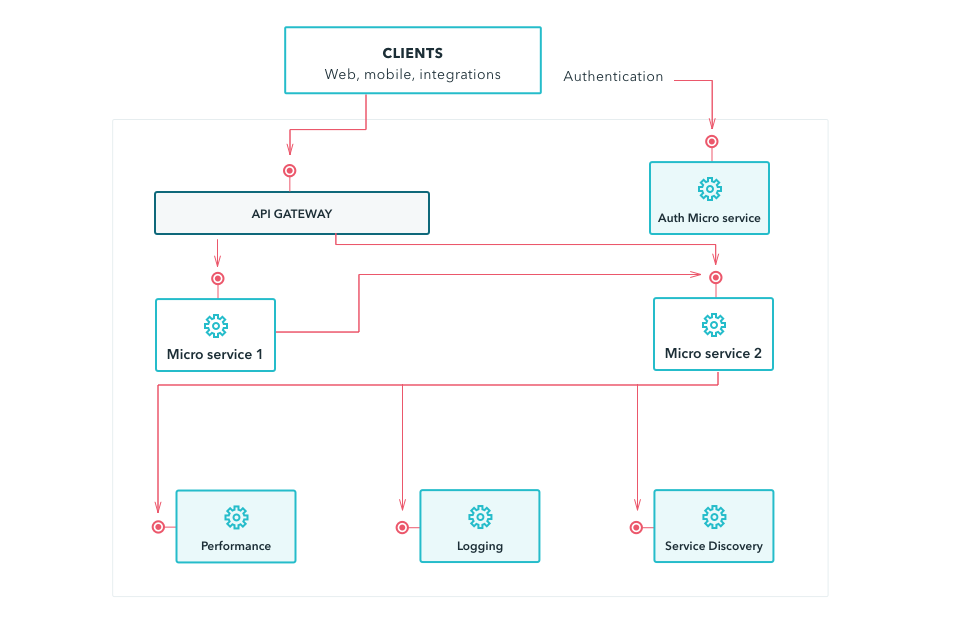
\includegraphics[width=10cm]{5.png}
	\caption{Een microservice dat een gateway gebruikt. \textcite{Benetis2016}}
	\centering
\end{figure}

Nu is er al een deftige architectuur aanwezig. Stap 6, "construct events", zal het plaatje dan ook compleet maken. De meeste microservices vragen aan asynchrone oplossing. Een niet-gelijktijdige verwerking van aanvragen. Een manier om asynchroon te werken, is werken met een queue of wachtrij. Een bekende manier om asynchroniteit toe te passen is publish/subscribe pattroon. Dit wil zeggen dat microservice A zijn berichten of data op een wachtrij gaat zetten. De microservices die data of berichten van microservice A moeten ontvangen, gaan zich abonneren op die wachtrij. Dus vanaf het moment dat microservice A iets op die wachtrij plaatst, krijgen de geabonneerden een melding en kunnen ze het bericht of de data gaan ophalen. Enkele voordelen van dit als asynchrone oplossing te gebruiken:
\begin{itemize}
	\item Taken inplannen. Dit kan door deze gewoon op de wachtrij te plaatsen met een timestamp van wanneer deze moet gebeuren of door een wachtrij te maken voor geplande events.
	\item Abonneren op bepaalde events.
	\item Het asynchrone systeem laten bloot leggen zodat externe klanten verschillende notificaties kunnen handelen.
\end{itemize}
In figuur 2.7 wordt de volledige architectuur weergegeven. Daar wordt er ook mooi afgebeeld hoe men events pland. Als event A voor event B moet gebeuren dan zetten ze die zo op de wachtrij event A voor event B. Want een wachtrij werkt volgens het FIFO (first in first out) principe.
\begin{figure}[h]
	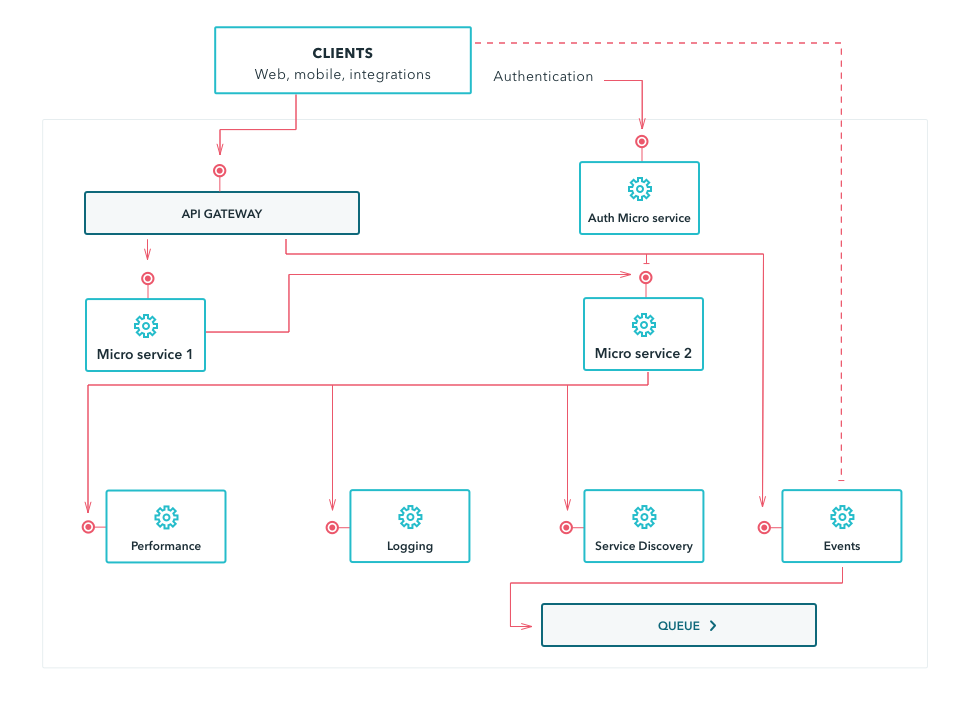
\includegraphics[width=10cm]{6.png}
	\caption{Een microservice met asynchronisatie. \textcite{Benetis2016}}
	\centering
\end{figure}

\textcite{Benetis2016a} beschrijft dat over volgende puntjes goed moet worden nagedacht voordat men de overschakeling maakt naar microservices:
\begin{itemize}
	\item Heeft de organisatie de microservice architectuur wel nodig?
	\item Zijn de juiste competenties aanwezig? Microservices zijn in het algemeen complexer dan een monolithic. Zeker omdat dit iets nieuws is. 
	\item  Staat iedereen achter deze verandering?
\end{itemize}
Eens de beslissing gevallen is om over te schakelen, moet er beslist worden hoeveel de infrastructurele vernadringen van de scope inpalmen. Het verloop om microservices te creëeren gaat als volgt in dit artikel. Eerst het uit elkaar trekken van het bestaande systeem, om het dan in microservices te steken, is een goed begin. Zo moet er constant nagedacht worden over de algemene infrastructuur. Een groot valluik in het begin van het proces is een proof of concept maken. Dit eindigt meestal in een infrastructuur dat niet overeenkomt met de waarden van microservices. Het probleem ligt dan meestal bij een onduidelijke scope. De business requirements zijn meestal wel duidelijk, dit geldt dan meestal niet voor niet-functionele requirements. Daarnaast moeten ook nog volgende stappen gerealiseerd worden:
\begin{itemize}
	\item Bescherming.
	\item Deployment automatisatie.
	\item Loggen en monitoren van microservices hun gedrag.
\end{itemize}
Velen komen niet tot deze stap, door de onderschatting van de overschakeling naar microservices.


\subsection{De voordelen en nadelen van microserivces}
In het artikel van \textcite{series2018} wordt er veel lofzang gedaan over microservices. Het gebruik van microservices zou ervoor zorgen dat de architectuur flexibeler wordt. Met flexibeler wordt bedoelt dat de architectuur zich kan 'aanpassen' of kan inspelen op verschillende situaties. Er kunnen microservices hergebruikt worden. Dankzij microservices is het hermodeleren, implementeren van nieuwe technologieën, ... 
Kleinere deeltjes zijn gemakkelijker te documenteren. De snelheid van microservices zijn een groot pluspunt. Hiermee wordt er geprobeert om aan te halen dat microservices sneller reageren omdat zo kleine, onafhankelijke services zijn. Ze moeten geen 'onnodige' stappen maken om de wens van de klant te vervullen. 
\textcite{Watts2018} geeft enkele voordelen van een microservice. Een developer is onafhankelijk. Ze hebben vrijheid. Ook het scalen van een microservice is veel eenvoudiger. Dit komt door dat microservices minder resources nodig hebben dan een volledige monolithic. Resources zijn hulpbronnen. Zoals al vaak aangehaald in deze bachelorproef, zijn microservices onafhankelijk en zouden ze daarom ook geen hulpbronnen nodig mogen hebben. Binnen een monolithic zijn deeltjes afhankelijk van elkaar en hebben elkaar dus nodig om goed te kunnen functioneren. De deeltjes binnen de monolithic hebben elkaar dus nodig en mogelijk als hulpbron. Een ander voordeel is bij het falen van een microservices, de andere microservices er geen last van zullen hebben. Dit komt door hun onafhankelijkheid. 
\textcite{Benetis2016} geeft aan dat volgende puntjes voordelen zijn van microservices:
\begin{itemize}
	\item Sneller en gemakkelijker developen.
	\item Het refactoren van deeltjes is eenvoudiger door de onafhankelijkheid van de services. 
	\item De schaalbaarheid is eenvoudiger dan bij een monolithic. We kunnen microservices gewoon 'klonen' of kopieëren. 
	\item Het deployen van een onderdeel gaat sneller omdat het team gespecialiseerd is in die bepaalde service.
	\item Als er iets faalt dan is de impact veel kleiner dan bij een monolithic. Dit komt ook door de onafhankelijkheid van de services. 
\end{itemize}
Maar om ervoor te zorgen dat dit allemaal vlot verloopt moeten er ook aanpassingen binnen in het bedrijf/ de organisatie gebeuren. 
\begin{itemize}
	\item Een project zal ingedeeld moeten worden in kleine requirements. De scope zal gedetailleerder moeten zijn.
	\item De teams zullen kleiner moeten worden gemaakt. Zodat er meer op de Agile methode kan gewerkt worden. 
	\item Er zal een sterke band komen met DevOps. Dit komt omdat veel services volledige automatische deployment vragen.
	\item Ook de communicatie tussen de services zal beter moeten worden uitgedacht.
	\item Documenteren is belangrijk. Dit is niet enkel het geval voor microservices maar ook voor elk project.
\end{itemize}

Enkele nadelen en moeilijkheden, \textcite{Koukia2018}:
\begin{itemize}
	\item Distributed systems are complex. Microservices vragen meer werk. Dit komt omdat het een nieuwere technology is en het concept is niet altijd meteen duidelijk. 
	\item Complexiteit is er overal. Een monolithic bevat ook complexiteit, maar wel een bekende complexiteit. Als er al een tijdje gewerkt wordt met monolithic, dan is die complexiteit een bekende eigenschap van de architectuur. Omdat microservices iets nieuws is, komt er complexiteit die minder bekend is onder de developers.
	\item Debuggen en fouten vinden is moeilijker. Bij een monolithic is het eenvoudig, bij aanpassingen wordt de volledige architectuur gerund. Als de gehele architectuur bij een microservices moet getest worden. Hier werd in het vorige deel meer uitleg over gegeven.
	\item Bij aanpassingen binnen een monolithic moest er maar één request gedaan worden om code samen te voegen. Bij microservices is dit verschillend. Er moet bijvoorbeeld in vier microservices iets aangepast worden voor een nieuwe feature. Dan moeten er vier requests verstuurd worden om die code te mergen. Want de services binnen de microservice architectuur zijn onafhankelijk van elkaar. 
\end{itemize}

\section{Order-to-cash proces in SAP}
\subsection{Definite}
\textcite{Wong2018} legt uit wat een order-to-cash proces inhoudt. Dit proces heeft veel invloed op het succes van een bedrijf. Ook het het veel invloed op de relatie met de klant. Een voordeel met de huidige technologie is dat het mogelijk is om het proces volledig te automatiseren. Dit heeft veel zorgt voor een minimaal aan fouten en vertragingen. Ook de data en gegevens die worden opgehaald en geanalyseerd is correcter. 
Het proces begint bij het plaatsen van een order door de klant. Alles wat ervoor zorgt dat de klant een order plaatst behoort tot branding, marketing of sales. De hoofdactiviteit van deze afdelingen ligt bij customer relationship, iets wat plaatsvindt voor het OTC proces. Het maakt er geen deel van uit. 
Velen denken dat een OTC is afgerond wanneer de inning heeft plaatsgevonden. Maar er zijn nog belangrijke stappen die gebeuren na het innen van het geld. Onder andere de data die verzameld is tijdens het proces moet geanalyseerd worden om zo het proces te optimaliseren. 
\begin{figure}[h]
	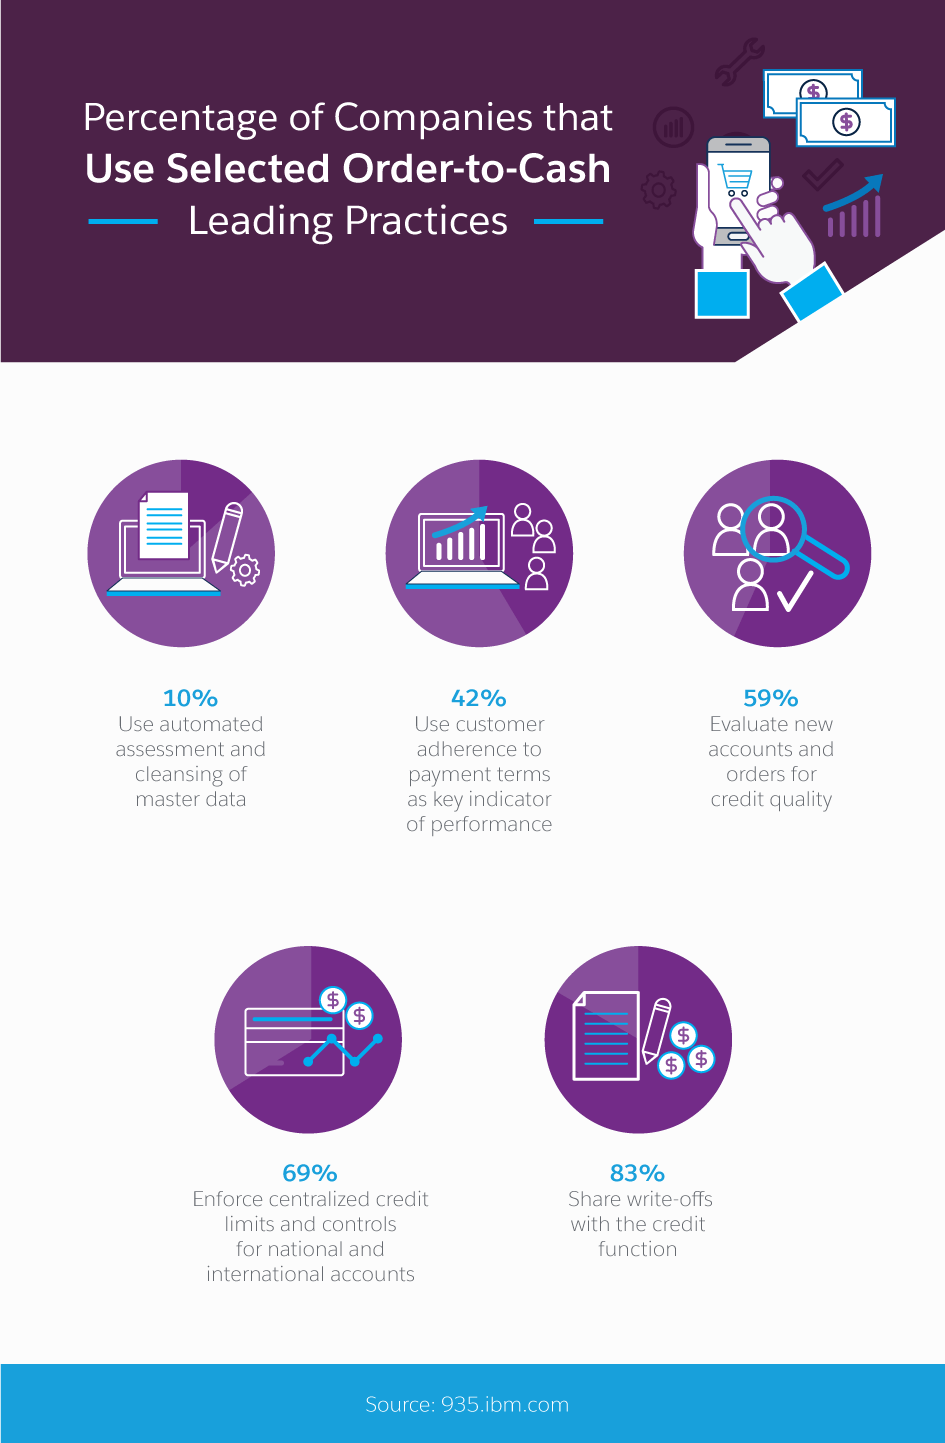
\includegraphics[width=10cm]{wong.png}
	\caption{Het percentage van van bedrijven dat gebruik maken van order-to-cash proces. \textcite{Wong2018}}
	\centering
\end{figure}
Het OTC proces heeft invloed op volgende delen van het bedrijf:
\begin{itemize}
	\item Supply chaing management
	\item Voorraadbeheer
	\item Human resources
	\item Financiële afdeling
\end{itemize}
Zijn er problemen in één van die afdelingen, kan dit voor vertraging zorgen in de andere afdelingen. Bij vertragingen van betalingen of inningen kan zorgen voor een minder goede cash flow binnen het bedrijf. 
Een goed OTC proces maakt indruk op de buitenwereld. Doordat het OTC goed gemanaged wordt, wordt er een beeld gecreërd dat het bedrijf stabiel is. 
Ook bij een OTC is technologie cruciaal. Elk deeltje van het proces kan beter worden door de nieuwe technologie. Er zijn verschillende onderdelen nodig om het proces te optimaliseren om accurate en real-time informatie te verkrijgen. Zoals: 
\begin{itemize}
	\item Gegevens die onderling verbonden zijn.
	\item Automatisering
	\item digitale facturatie
	\item Digitale verzending van het management.
\end{itemize}

Volgende acht stappen komen voor in een OTC proces:
\begin{itemize}
	\item Order management
	\item Credit management
	\item Order fulfillment
	\item Order shipping
	\item Facturatie
	\item Accounts receivable
	\item Inning van het geld
	\item Rapportering en data management
\end{itemize}
In figuur X wordt het afgebeeld in een schema.
\begin{figure}[h]
	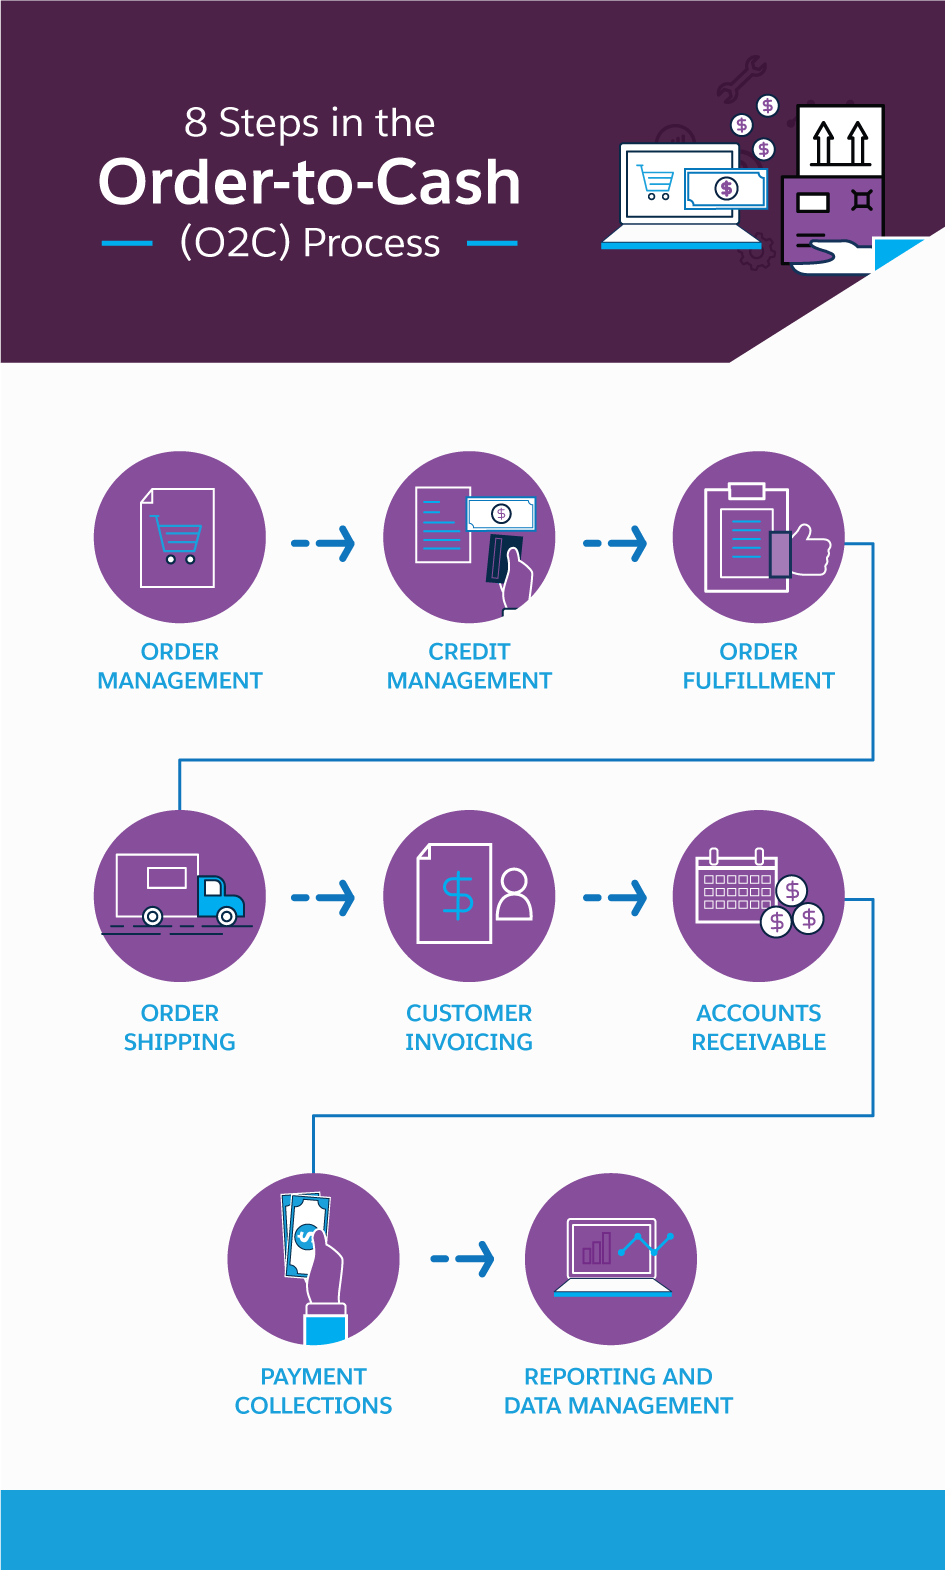
\includegraphics[width=10cm]{wong2.png}
	\caption{Het order-to-cash proces. \textcite{Wong2018}}
	\centering
\end{figure}
Order management is de eerste stap in het proces. Dit begint wanneer de klant een order plaatst. De manier waarop is niet zo belangrijk. Dit deeltje van het proces moet geautomatiseerd zijn. Bij het plaatsen van een order, moet er een ander onderdeel van het order proces getriggerd worden. Dit moet ervoor zorgen dat het order niet uit het oog verloren wordt. Door de automatisatie worden de andere deelnemende partijen direct ingelicht over het nieuwe order en dit heeft een voordeel als het op tijdig leveren aankomt.
Hierna komt credit management. Dit moet ervoor zorgen dat er minder problemen zijn op het einde van het proces. Credit management houdt in dat men kijkt naar hoe het betalingsgedrag van de klant is geweest. Zijn er nog openstaande facturen, betaald de klant altijd maar na enkele aanmaningen? Door dit gedeelte te automatiseren, kan er bespaard worden op menskracht en geld. Als er toch dieper moet gekeken worden naar het betaalgedrag van een klant, kan dit doorgestuurd worden naar een werknemer die er dan naar kijkt. Maar dat zouden dan enkele klanten hun betaalgedrag moeten nagekeken worden, i.d.p.v. alle klanten die een order plaatsen. 
De klanten die een goed betaalgedrag vertonen, worden doorgestuurd naar de volgende stap: Order fulfillment. In deze stap wordt het order ook echt samengesteld en uit de 'rekken' gehaald. Het is een groot voordeel als ook dit gedeelte geautomatiseerd is. Bij het verkopen van een product moet de voorraad automatisch aangepast worden. Eens de producten van het order samengebracht zijn gaan we over naar de volgende stap, order shipping. De verzending van de goederen. De verzending moet goed opgevolgd worden om mogelijke vertragingen te minimaliseren. De gegevens die vrijkomen bij een verzending, moeten zo snel mogelijk in het systeem worden ignegeven. Zodat ook dit deeltje van het proces geoptimaliseerd kan worden. 
Na het verzenden van de goederen komt de facturatie. Op dit deeltje heeft credit management veel invloed. Doordat de wanbetalers er in stap twee al zijn uitgehaald, zouden er hier minder problemen voorkomen. Als er hier fouten worden gemaakt, kan dit een sneeuwbal effect veroorzaken. Dit betekend dat één fout een andere fout kan triggeren en zo voorts. Het systeem moet de juiste info verkrijgen van de werknemers. De info bevat meestal volgende puntjes:
\begin{itemize}
	\item Order specificaties
	\item De kosten
	\item Credit terms
	\item Order datum
	\item Verzendingsdatum
\end{itemize}
Die puntjes moeten ingevoerd worden zodat het facturatiesysteem geautomatiseerd kan worden. Zodat ook hier vertragingen en fouten kunnen geminimaliseerd worden. Eens de factuur is uitgestuurd, wordt er een betaling verwacht binnen een bepaalde periode. Het systeem zou dit ook moeten bijhouden en ervoor zorgen dat er een melding gestuurd wordt nog voor de betalingsperiode is afgelopen. Dit valt onder de volgende stap accoutns receivable. Deze stap probeert om te voorkomen dat mensen vergeten te betalen. 
De volgende stap is payment collections. Wordt een factuur niet betaald binnen de gevraagde periode dan wordt er een aanmaning gestuurd en wordt dit ook in het systeem bijgehouden. De werknemers moeten ook de klanten contacteren zodat ze een reden kunnen geven voor het mogelijks vergeten van de betaling. 
Als laatste stap komt reporting en data management aan bod. Er bestaan programma's om ervoor te zorgen dat performance data over elk deeltje van het proces wordt opgehaald. Door achteraf deze data te gaan analyseren, kan er veel duidelijkheid komen van waar het verkeerd loopt. 

\textcite{PEARSON2017} beschrijft waarom het zo belangrijk is om een goed OTC proces te hebben. Vroeger waren de eisen van de klanten minder hoog. Als klanten iets bestellen, willen ze het de volgende dag al in huis hebben. Er zijn ook voor- en nadelen aan een OTC proces. Als het proces goed opgezet is, kan dit zorgen voor blijere klanten, minder wanbetalers, ... 

Maar is het order management proces niet goed opgezet dan kan het heel snel slecht gaan. Klanten zullen niet tevreden zijn. 
Veel voorkomende redenen van ontevreden klanten:
\begin{itemize}
	\item Orders zitten er dubbel in.
	\item Er zit vertraging tussen de verschillende onderdelen van het proces.
	\item De levering klopt niet met wat er gefactureerd wordt.
	\item Een slecht voorraadbeheer waardoor niet aan de beloften zoals leveringstijd kan voldaan worden.
\end{itemize}
Om zulke problemen op te lossen moet men eerst gaan zoeken van waar die problemen komen. Automatisering is hier een goede oplossing voor. Dordaat verschillende processen aan elkaar gelinkt zijn, is er minder ruimte voor vertragingen. Enkele best practices omvatten:
\begin{itemize}
	\item Minimaliseren van werknemers die handmatig gegevens moeten invullen.
	\item Klanten de mogelijkheid geven om hun bestellingen online te maken.
	\item Integratie van de informatie over het gehele proces.
	\item Elimineren van onnodige moeilijkheden binnen in het proces.
\end{itemize}

Ook het tweede subproces, bill-to-cash proces, heeft pitfalls en best practices.
In volgende opsomming komen verschillende signalen aan bod waaraan te zien is dat het bill-to-cash proces niet goed in elkaar zit.
\begin{itemize}
	\item Het aantal verkoopsovereenkomsten met speciale eisen van de klant is groot. bivjoorbeeld meer dan de helft heeft een uniek verkoopsovereenkomst.
	\item Herhalend aanbiedingen en toegevingen moeten doen door fouten in het proces.
	\item Wat op dee oorspronkelijke offerte stond, werd niet gefactureerd, er werd meer aangerekend.
	\item Een groot aantal creditnota's uitgegeven.
	\item Tussen de verkoop, verzending en het facturerings proces zitten informatie gaten.
\end{itemize}
Om dit alles weg te werken moet er goed gekeken worden naar waar de problemen nu zitten. Enkele best practices:
\begin{itemize}
	\item Integreer klantenprofielen in de betalingssoftware.
	\item Integreer de facturatie en betalingsgegevens met elkaar zodat op de factuur de juiste betalingsmethode staat.
\end{itemize}


\subsection{Technologie}
\subsubsection{Onderdelen van een order-to-cash proces}
Er zijn vier grote onderdelen, namelijk:
\begin{itemize}
	\item Voor-verkoopsactiviteiten.
	\item Het order proces.
	\item Order afwerking.
	\item Betaling.
\end{itemize}
Bij de voor-verkoopsactiviteiten verstaan we het contact dat moet worden gemaakt worden met klant. De klant moet overtuigd worden van het product. Na contact komt er al dan niet een offerte. Soms kan er ook van contact rechtstreeks naar een order gaan. 
Het orderproces bevat maar één onderdeel namelijk: de sales order. 
Binnen de order afwerking valt het leveren van goederen, het verzenden van goederen.
\textcite{Kumaran2015} geeft een mooi overzicht van de stappen die een order to cash proces kan bevatten. Zo begint het artikel met een toelichting dat dit proces een core proces is van de business. Dit wil zeggen dat een bedrijf, zonder dit proces, geen winst kan maken. Het is een essentieel onderdeel van zo wat elk bedrijf. Hoe deze vorm krijgt binnen een bedrijf, is heel verschillend. Een OTC proces start met het ontvangen van orders. Daarna kan, dit gebeurt niet overal, er gekeken worden naar het krediet van de klanten. Mag deze klant wel nog een bestelling plaatsen? Hierna wordt het order opgenomen in het systeem. Het product wordt verzonden en geleverd. En als laatste wordt de factuur betaald. Dit is welliswaar het 'perfecte' verloop van een order to cash proces. 
\begin{figure}[h]
	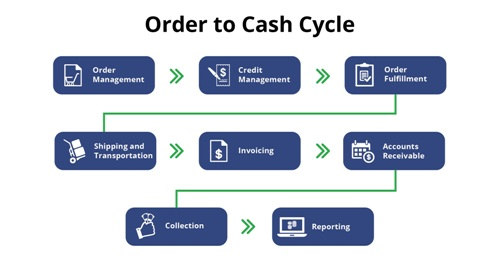
\includegraphics[width=10cm]{Order-to-cash-cycle.jpg}
	\caption{Order-to-cash proces volgens \textcite{Kumaran2015}.}
	\centering
\end{figure}
Er zijn ook enkele uitdagingen verbonden met dit proces. In de volgende opsomming vindt je er enkele:
\begin{itemize}
	\item Hou de orders goed bij, anders loopt het fout vanaf het begin. 
	\item Zonder automatisering verlies je veel tijd. Kostbare tijd.
	\item Zorgen dat de logistiek 'on point' is, is heel belangrijk. Dit is een belangrijk onderdeel binnen het proces.
	\item Bij wanbetalingen, moet de customer service ingrijpen. Ook zij zijn een belangrijk onderdeel van het proces.
\end{itemize}
Het managen van een OTC proces is even belangrijk als de andere aspecten. Een slecht gemanaged proces kan op lange termijn duurder uitkomen dan een onderdeel dat nog niet geautomatiseerd is. 

\textcite{PEARSON2017} vindt dat een OTC proces bestaat uit twee subprocessen. Het order managmenet proces en het bill-to-cash proces. Het laatst vernoemde proces gaat over de facturatie en de inning van het geld.

\textcite{2019} geeft meer uitleg bij enkele termen die in SAP voorkomen. Bij het proces is er een sales team aanwezig. Die spreken met de klant en maken afspraken. Zij zorgen ook voor een deal met de klant. Zij hebben toegang tot informatie over de klant, producten, kwaliteit, prijzen, etc. 
Om ervoor te zorgen dat een order kan verzonden worden, moeten de goederen  opgehaald worden. Die goederen worden opgeslaan in een magazijn. Daar wordt aan order picking en packing gedaan. Bij picking gaat men gaan kijken naar de voorraad om de order te kunnen opvullen. Packing gaat over het inpakken van de goederen tegen beschadigingen. Dit kan door allemaal dozen op een pallet te zetten. Eens de goederen door de fase picking en packing zijn geweest, komt het laden voor transport. De goederen worden dan in containers geladen om dan te verzenden via vrachtwagen of per boot. Hierna komt de facturatie. Dan moet er gewacht worden op de betaling van de klant. Bij laattijdige betaling worden er aanmaningen gestuurd. 
\begin{table}[]
	\resizebox{\textwidth}{!}{%
		\begin{tabular}{|l|p{10cm}|}
				\hline Delivery document & Dit is het leveringsdocument dat gekoppeld is aan een order. Dit wordt uitgestuurd om te bewijzen dat het order geleverd is. \\ \hline
			Picking & Het nagaan of de goederen in de voorraad zitten en ze ook gaan ophalen uit het magazijn. \\ \hline
			Packing & Het inpakken van goederen in dozen, containers, palletten. \\ \hline
			Loading & De goederen inladen in de vrachtwagen of de container. \\ \hline
			Shipment document & Dit document wordt mee afgeleverd met de goederen. Het kan als een soort checklist dienen om na te gaan of alles wel in het afgeleverd pakket zit. \\ \hline
			Shipment cost document & Hierop is de kost terug te vinden van het transport. \\ \hline
			Customer billing document & Dit is een verkoopsdocument, dus dit moet de klant niet betalen. Dit document refereerd naar het delivery document. \\ \hline
			Customer invoice & Dit is de factuur die de klant opgestuurd krijgt. \\ \hline
		\end{tabular}%
	}
	\caption{Tabel met uitleg over termen. \textcite{2019}}
\end{table}


\subsubsection{Wat biedt SAP zelf aan voor microservices}
\textcite{Kyma2019} verteld hoe Kyma in elkaar zit. Dit is een recent project van SAP om toenadering te geven toto microserivces. Kyma is een open-source project gemaakt om Kubernetes. Kubernetes wordt gebruikt om applicaties op verschillende machines te managen. Je kan hiermee cloud-based applicaties en on-premise applicaties omzetten naar een microservice architectuur of naar serverless computing. Cloud-based applicaties zijn applicaties die hun data gaan ophalen over het internet in de plaats van op de harde schijf van de computer. On-premise applicaties zijn de tegenhangers van cloud-based. On-premise is lokaal op de computer, op de harde schijf. Serverless computing gebeurt in de cloud. Dit zorgt ervoor dat er op een dynamische manier de resources van een machine kan aangepast worden. 
Kyma zorgt voor betere end-to-end ervarings scenario's. Die volgen een best-practices voor performance, schaalbaarheid, efficentie en beveiliging. 

\textcite{Semerdzhiev2018} geeft een introductie in het project Kyma van SAP. Binnen SAP wordt er omgegaan met software van verschillende leveranciers. SAP probeert om hun software te customizen naar de wensen van de klant. Dit vraagt meer openheid en een modernere architectuur. 
Het idee achter Kyma is het creëeren van serverless applicaties, mashups en microservices. Ook kan het gebruikt worden om snel kleine, gecustomizede modules te developen. Die modules zijn dan verworven met business logica. 
Er werd iets zoals Knative gemaakt. Knative is een platform dat developers ondersteund om serverless applicaties te maken op Kubernetes. Dit zorgde voor groot enthousiasme bij SAP omdat hun Kyma project een soort van bevesteging keer. Al snel werd Kyma gerefactored om samen te kunnen werken met Knative. Er werden overlappende componenten weggelaten, wat Kyma slanker en gestroomlijnder maakt. Dankzij Knative kan Kyma zich richten op higer-level enterprise applications en service consumption scenario's. En gebruik maken van Knative voor de infrastructuur en development scenario's. 

\textcite{Hofmann2018} geeft het update over de integratie tussen Kyma en Knative. Een toch redelijk belangrijke samenwerking. Beide bieden een complete set van bouwblokken aan. Beiden zijn ook een sterk framework. Bij het gebruik van beide kunnen er could-native oplossingen gebouwd worden op Kubernetes met een sterk framework. Op figuur X is te wat Kyma en wat Knative aanbiedt. 
\begin{figure}[h]
	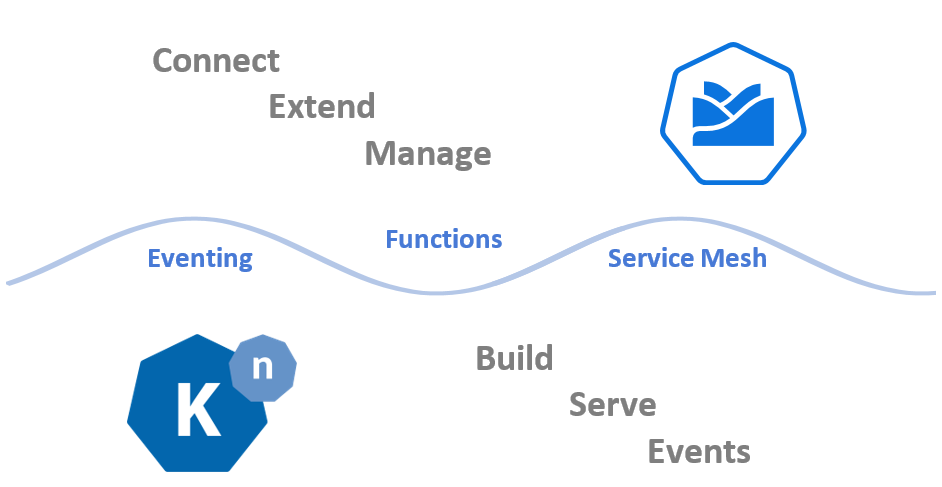
\includegraphics[width=10cm]{1-kyma-knative.png}
	\caption{Wat Kyma, boven de lijn, aanbiedt en wat Knative, onder de lijn, aanbiedt \textcite{Hofmann2018}.}
	\centering
\end{figure}
De laatste maanden werden de repositories gereconstrueerd en daarom zijn er geen tot weinig referenties naar Knative. Naast die grote verandering werd er gewerkt aan een proof-of-concept cloud-native oplossing door het gebruik van Knative en Kyma te samen. 

Kyma heeft hard gewerkt om deze problemen/uitdagingen te proberen wegwerken. Kyma heeft ook geprobeerd om bedrijven te helpen met de transformatie naar digitalisatie. Kyma geeft bedrijven de mogelijkheid tot:
\begin{itemize}
	\item Be open and extendable: Kyma maakt gebruik van Open Service Broker API specificaties. Dit is een "plug and play" die de mogelijkheid geeft om code te hergebruiken. Ook code van andere partijen te gebruiken. 
	\item Be seamlessly connected: Een eenvoudige manier om een beveiligde connectie te hebben tussen systemen. Deze kunnen gemanaged worden binnen de huidige applicatie om oplossingen te maken in hetrogene landschappen. Eén connectie geeft veel mogelijkheden.
	\item Use any programming language: Developers kunnen in hun geweste programmeertaal coderen.
	\item Bring speed and agility: Er moet niet maanden gewacht worden om use cases of functionaliteiten op te leveren. 
	\item Accelerate innovation: Meestal start dit als een test of een trail. Bij zulke scenario's zijn de kost en de snelheid van zeer groot belang. Dankzij Kyma kunnen bedrijven meteen beginnen werken aan een oplossingen en moet er geen tijd besteed worden aan het zoeken van de best mogelijke oplossing. 
\end{itemize}


\section{Requirements van de business}
\textcite{Biedron2018} legt uit wat een order to cash proces is. Daaruit kunnen we volgende requirements uit afleiden:
\begin{itemize}
	\item De klant moet een order of meerdere orders kunnen plaatsen. Een goed werkend order-systeem is een must.
	\item De order ophalen uit de voorraad. Er moet een goed voorraad beheer aanwezig zijn. Dit moet ervoor zorgen dat het aantal laattijdige leveringen geminimaliseerd wordt. Samen met het goede voorraadbeheer wordt ook best bijgehouden waar je je goederen geplaatst hebt in je magazijn.
	\item De levering moet goed gepland worden. Dit zou voor het grootste deel al geautomatiseerd moeten zijn. Een email met informatie over de levering is een must. 
	\item Aanmaken van een factuur op basis van het geplaatst order met de juiste klantgegevens zou een geautmatiseerd onderdeel moeten zijn. 
	\item De betaling van de factuur komt toe in de financiele afdeling. Automatische afhandeling is een must.
\end{itemize}
Bij een order plaatsen komen volgende elementen aanbod:
\begin{itemize}
	\item Er moet een lijst met producten beschikbaar zijn.
	\item De klant zijn gegevens moeten gekend zijn bij het bedrijf.
	\item Het systeem bij het bedrijf moet beschikbaar zijn.
\end{itemize}
Na het plaatsen van de order moet die ook klaargezet worden om te leveren. Daar zijn volgende elementen van belang:
\begin{itemize}
	\item Een goed voorraadbeheer is de eerste must.
	\item Een overzicht van waar alles staat, geeft ook een meerwaarde.
	\item Bij het ophalen van een product om bij een order te plaatsen, moet de hoeveelheid in de voorraad verminderen.
\end{itemize}
